\documentclass[twoside,a4paper,article]{combine}

\usepackage[latin1]{inputenc}
\usepackage{a4}
\usepackage{fancyhdr}   
\usepackage{makeidx}
\usepackage{color}
\usepackage{t1enc}
\usepackage{latexsym}
\usepackage{amssymb}
\usepackage{amsmath}
\usepackage{subfigure}

\usepackage{graphicx}
\usepackage{pslatex}
\usepackage{ifthen}

\usepackage[T1]{fontenc}
\usepackage{pslatex}

\usepackage{psfrag}
\usepackage{url}

\usepackage{enumerate}
\usepackage{amsmath}

\usepackage{ntheorem}
\theoremstyle{break}
\newtheorem{algorithm}{Algorithm}[section] 

\usepackage[font={small}]{caption}
\usepackage{paralist}
\usepackage{sidecap}
\usepackage{subfigure}
\usepackage{tikz}
\usepackage{pgfplots}
\usetikzlibrary{fadings}

\usepackage{titlesec}
\usepackage{titling}

\setcounter{secnumdepth}{4}

\titleformat{\paragraph}
{\normalfont\normalsize\bfseries}{\theparagraph}{1em}{}
\titlespacing*{\paragraph}
{0pt}{3.25ex plus 1ex minus .2ex}{1.5ex plus .2ex}

\setlength{\oddsidemargin}{3.6pt}
\setlength{\evensidemargin}{22.6pt}
\setlength{\textwidth}{426.8pt}
\setlength{\textheight}{654.4pt}
\setlength{\headsep}{18pt}
\setlength{\headheight}{15pt}
\setlength{\topmargin}{-41.7pt}
\setlength{\topskip}{10pt}
\setlength{\footskip}{42pt}

\setlength{\parindent}{0pt}

\setcounter{secnumdepth}{3}
\setcounter{tocdepth}{3}

\usepackage{xspace} % context sensitive space after macros
\makeatletter
\DeclareRobustCommand\onedot{\futurelet\@let@token\@onedot}
\def\@onedot{\ifx\@let@token.\else.\null\fi\xspace}
\def\eg{{e.g}\onedot} \def\Eg{{E.g}\onedot}
\def\ie{{i.e}\onedot} \def\Ie{{I.e}\onedot}
\def\cf{{c.f}\onedot} \def\Cf{{C.f}\onedot}
\def\etc{{etc}\onedot} \def\vs{{vs}\onedot}
\def\wrt{w.r.t\onedot} \def\dof{d.o.f\onedot}
\def\etal{{et al}\onedot}
\def\zB{z.B\onedot} \def\ZB{Z.B\onedot}
\def\dh{d.h\onedot} \def\Dh{D.h\onedot}

% http://tex.stackexchange.com/questions/5223/command-for-argmin-or-argmax
\DeclareMathOperator*{\argmin}{arg\,min}

\makeglossary

\begin{document}
	\begin{titlepage}
	\begin{center}
		\ 
		\vspace{3.5cm}


		\textsf
		{
		Fakult\"at f\"ur Mathematik, Informatik und Naturwissenschaften\\
		Lehr- und Forschungsgebiet Informatik VIII\\
		Computer Vision\\
		Prof. Dr. Bastian Leibe
		}

		\rule{\linewidth}{1pt}

		\vspace{1.75cm}
		\LARGE
		\textbf{Seminar Report}

		\vspace{1.7cm}
		\huge Neural Codes for Image Retrieval

		\vspace{3.0cm}
		\Large David Stutz\\
		\Large Matriculation number: \#\#\#\#\#\#

		\vspace{0.5cm}
		\today

		\vspace{1.05cm}
		\rule{\linewidth}{1pt}

		\vspace{0.5cm}
		\textsf{
			\textbf{
				\normalsize
				\begin{tabular}{ll}
					Advisor:  & Michael Kramp\\
				\end{tabular}
			}
		}
	\end{center}
\end{titlepage}


	\begin{abstract}
	This seminar report focuses on using convolutional neural networks for image retrieval. Firstly, we give a thorough discussion of several state-of-the-art techniques in image retrieval by considering the associated subproblems: image description, descriptor compression, nearest-neighbor search and query expansion. We discuss both the aggregation of local descriptors using clustering and metric learning techniques as well as global descriptors.
	
Subsequently, we briefly introduce the basic concepts of deep convolutional neural networks, focusing on the architecture proposed by Krizhevsky \etal \cite{KrizhevskySutskeverHinton:2012}. We discuss different types of layers commonly used in recent architectures, for example convolutional layers, non-linearity and rectification layers, pooling layers as well as local contrast normalization layers. Finally, we shortly review supervised training techniques based on stochastic gradient descent and regularization techniques such as dropout and weight decay.

Finally, following Babenko \etal \cite{BabenkoSlesarevChigorinLempitsky:2014}, we discuss the use of feature activations in intermediate layers as image representation for image retrieval. After presenting experiments and comparing convolutional neural networks for image retrieval with other state-of-the-art techniques, we conclude by motivating the combined use of deep architectures and hand-crafted image representations for accurate and efficient image retrieval.
\end{abstract}


	\tableofcontents
	\newpage

	\section{Introduction}

Content-based image or object retrieval,
% \footnote{
    % The difference between object retrieval and image retrieval is given implicitly within the literature and techniques can often be used for both problems (for example see \cite{PhilbinChumIsardSivicZisserman:2007}). Further, the term object may be inappropriate when referring to scenes instead of single objects. Therefore, in the following, we speak of image retrieval and often refer to these subproblems implicitly. In addition, we always refer to content-based image retrieval (that is no meta information is used).
% }
the problem of finding images within a large database containing the same or similar objects or scenes as a given query image, is a fundamental problem in computer vision. In particular, in order to extract useful information from large databases of images these databases need to be organized and searchable.
% The problem arises from the wish to extract information from large databases of digital images. However, information may only be extracted when the data can be organized efficiently \cite{RuiHuangChang:1999}.
Originally, images were manually annotated with keywords and text-based retrieval systems were utilized. However, due to the rapidly increasing size of image collections, manual annotation became infeasible. Therefore, content-based retrieval systems relying on image content only were developed and are heavily researched within the computer vision community.
% In practice, given a query image, the problem is often simplified by asking for an ordered list of images containing the same object or showing a similar scene with high probability \cite{PhilbinChumIsardSivicZisserman:2007}.
% A formal definition of the problem is given in section \ref{sec:image-retrieval}.
In the following, we always speak of content-based image retrieval and include the subproblem of object retrieval implicitly (in practice, techniques can often be applied to both problems \cite{PhilbinChumIsardSivicZisserman:2007}).

While the problem has been studied for several decades, recent success is based on the Bag of Visual Words model proposed by Sivic and Zisserman \cite{SivicZisserman:2003}. Local descriptors, used to characterize interest points within the image, are quantized into so-called visual words and the image is represented by the corresponding word counts. While the Bag of Visual Words model has steadily been improved (for example \cite{ChumPhilbinSivicIsardZisserman:2007,PhilbinChumIsardSivicZisserman:2007,ArandjelovicZisserman:2012}), different techniques of aggregating local descriptors (for example \cite{JegouDouzeSchmidPerez:2010,GeKeSun:2013,JegouZisserman:2014,PhilbinIsardSivicZisserman:2010}) have been used and global descriptors have been used, as well (for example \cite{OlivaTorralba:2001}).
% In analogy to the Bag of Words (BoW) model in text retrieval systems where a document is represented by a sparse vector counting word ocurrences, Sivic and Zisserman \cite{SivicZisserman:2003} proposed the Bag of Visual Words model. Using interest point detectors and local descriptors (see \cite{MikolajczykSchmid:2005}) the obtained feature vectors are quantized using clustering and an image is represented by the counts of word ocurrences. Since its introduction, the Bag of Visual Words model has steadily been improved (for example \cite{ChumPhilbinSivicIsardZisserman:2007,PhilbinChumIsardSivicZisserman:2007,ArandjelovicZisserman:2012}). Furthermore, different approaches of aggregating local descriptors have been proposed (for example \cite{JegouDouzeSchmidPerez:2010,GeKeSun:2013,JegouZisserman:2014}) and global descriptors have been used as well (for example \cite{DouzeJegouSandhawaliaAmsalegSchmid:2009}).

Similar to image retrieval, convolutional neural networks \cite{LeCunBoserDenkerhendersonHowardHubbardJackel:1989} have been studied for more than two decades (see \cite{Bengio:2009,LeCunBoserDenkerhendersonHowardHubbardJackel:1989}) but had their breakthrough only recently \cite{Bengio:2009}.
% Although such aggregation techniques show state-of-the-art performance, the underlying idea (inspired by the Bag of Visual Words model) is quite old now. 
% In contrast, onvolutional neural networks \cite{LeCunBoserDenkerhendersonHowardHubbardJackel:1989} had their breakthrough only recently.
In particular Krizhevsky \etal \cite{KrizhevskySutskeverHinton:2012} demonstrated astounding results on the ImageNet classification challenge
\footnote{
    See \url{http://www.image-net.org/challenges/LSVRC/2010/}.
}.
Thus, convolutional neural networks have been applied to a range of different applications, and the usefulness of the generated intermediate activations has been studied within the literature \cite{Bengio:2009}. Recently, Babenko \etal \cite{BabenkoSlesarevChigorinLempitsky:2014} used convolutional neural networks, in particular the architecture proposed by Krizhevsky \etal, for image retrieval.

\vskip 6px
\textbf{Outline.} This report is intended to introduce the reader to recent techniques in image retrieval. Furthermore, we briefly introduce the fundamentals of convolutional neural networks in order to discuss their application to image retrieval. In Section \ref{sec:image-retrieval} we introduce the problem of image retrieval and discuss aggregation techniques for local descriptors as well as the application of global descriptors. Furthermore, we briefly introduce approximate nearest neighbor techniques, discriminative dimensionality reduction and average query expansion. In Section \ref{sec:convolutional-neural-networks} we discuss the mathematical foundation of convolutional neural networks including their training and regularization. Subsequently, in Section \ref{sec:neural-codes-image-retrieval}, we discuss the application of convolutional neural networks for image retrieval before presenting experimental results by Babenko \etal. Finally, we conclude in Section \ref{sec:conclusion}.

% \subsection{Literature Notes}

% Unfortunately, to the best of our knowledge, no survey on image retrieval includes all or most of the approaches presented in this report. However, older surveys may introduce the reader to the field of image retrieval and discuss older techniques inspired by text retrieval (for example \cite{RuiHuangChang:1999}). Therefore, we refer the reader to some of the readings by Zisserman's group (for example \cite{SivicZisserman:2003,PhilbinChumIsardSivicZisserman:2007,ArandjelovicZisserman:2012}) and Schmid's group, especially work involving J{\'e}gou (for example \cite{JegouDouzeSchmidPerez:2010,ToliasAvrithisJegou:2013,JegouZisserman:2014}). Both groups maintain web pages providing datasets and software
% \footnote{
    % See \url{http://www.robots.ox.ac.uk/~vgg/software/}, \url{http://lear.inrialpes.fr/software}, \url{http://people.rennes.inria.fr/Herve.Jegou/index.html}.
    % Note that, at the point of writing, J{\'e}gou is not longer at LEAR INRIA.
% }.
% We also want to point the reader to a survey of local descriptors by Mikolajczyk and Schmid \cite{MikolajczykSchmid:2004} and note that their evaluation methodology is implemented in the VLBenchmarks library
% \footnote{
    % See \url{http://www.vlfeat.org/benchmarks/}.
% }.

% In contrast, several recent surveys on convolutional neural networks are available (for example \cite{Bengio:2009,Schmidhuber:2015}) and may introduce the reader to the necessary mathematical background and different applications.

	\section{Image Retrieval}
\label{sec:image-retrieval}

Given a database of images $X = \{x_1, \ldots, x_N\}$ and a query image $z_0$ showing a particular object or scene, the task of image retrieval is usually formalized as follows:

\vskip 6px
\textbf{Problem.} Find an ordered list of images $Z = (z_1, \ldots, z_K)$ such that, for an appropriate distance function $d$, it holds:
\begin{align}
    d(z_0, z_k) \leq d(z_0, z_{k + 1}), 1 \leq k < K\quad\text{ and }\quad d(z_0,z_k) < d(z_0, x_n) \forall 1 \leq k \leq K, x_n \notin Z\label{eq:nn}
\end{align}
which basically describes a $K$-nearest neighbor search.
\vskip 6px

% This formulation does summarize the usual approach taken towards image retrieval within the literature and reduces the original binary classification problem (for example ``find images containing the same object'') to a $Q$-nearest-neighbor problem \cite{PhilbinChumIsardSivicZisserman:2007}.

% In the following, we want to give a brief overview over different techniques employed for image retrieval. Beneath discussing approaches included in the comparison of Babenko \etal \cite{BabenkoSlesarevChigorinLempitsky:2014}, we discuss additional influential work and give a coarse taxanomy of these approaches.
% Roughly, we divide the image retrieval problem in image description, descripto compression and nearest-neighbor search and query expansion. While early work in image retrieval usually present complete image retrieval systems (see \cite{RuiHuangChang:1999}), recent publications focus on these subproblems.

While early work on image retrieval presented complete retrieval systems, recent publications usually focus on subproblems. Therefore, in the following, we roughly divide this problem into image description, compression, nearest neighbor search and query expansion.

\subsection{Image Description}

A fundamental problem in image retrieval is image representation, that is the characterization of an image using a feature vector of fixed dimensionality. We distinguish global descriptors directly constituting an image representation as well as local descriptors which usually need to be aggregated into an image representation of fixed dimensionality.

\subsubsection{Aggregation of Local Descriptors}
\label{subsubsec:local-descriptors}

Local descriptors are designed to represent regions around interest points. For image retrieval, these interest points are computed using a scale, rotation and affine invariant detector. 
% Usually, such detectors are developed to provide invariance towards rotation, scaling or affine transformation.
We refer to \cite{MikolajczykSchmid:2004} for details and discuss the Scale-Adapted Harris Detector as example~\cite{MikolajczykSchmid:2004}.

\vskip 6px
\textbf{Scale-Adapted Harris Detector} \cite{MikolajczykSchmid:2004,HarrisStephens:1988}. The Harris detector is based on the second moment matrix $A$
of an image $x_n$ (see Equation \eqref{eq:harris}).
%of the grayscale image $x_n$:
%\begin{align}
%    M = \begin{pmatrix}
%        \partial_x^2 x_n & \partial_x \partial_y x_n\\
%        \partial_x \partial_y x_n & \partial_y^2 x_n
%    \end{pmatrix}\label{eq:second-moment}.
%\end{align}
The corresponding eigenvalues $\lambda_1,\lambda_2$ represent the signal change in two orthogonal directions and interest points are extracted at pixels where both eigenvalues are large. For efficiency, Harris and Stephens \cite{HarrisStephens:1988} propose to maximize
\begin{align}
    \lambda_1 \lambda_2 - \kappa(\lambda_1 + \lambda_2)^2 = \text{det}(A) - \kappa \text{trace}(A)^2
    \quad\text{ with }\quad 
    A = \begin{pmatrix}
        \partial_x^2 x_n & \partial_{xy} x_n\\
        \partial_{xy} x_n & \partial_y^2 x_n
    \end{pmatrix}\label{eq:harris}
\end{align}
where $\kappa$ is a sensitivity parameter.
In practice, the detector is applied in scale space, that is on a set of images
\begin{align}
    x_n^{(\sigma_s)} = g_{\sigma_s} \ast x_n
\end{align}
where $\ast$ denotes convolution and $\sigma_s$ is sampled at logarithmic scale.
% \footnote{
    % The Gaussian scale space is given by a set of images $x_n^{(\sigma_s)} = g_{\sigma_s} \ast x_n$ with $\sigma_s$ usually sampled at a logarithmic scale.
% }
Therefore, it automatically selects the optimal scale and defines the size of the region used for local descriptors. Several extensions have been proposed, for example the Harris-Laplace Detector uses the Scale-Adapted Harris Detector to detect interest points in a coarse scale space, and then refines detections by searching for extrema of the Laplacian-of-Gaussians
\begin{align}
    \Delta (g_{\sigma_s} \ast x_n) = \partial_{xx} (g_{\sigma_s} \ast x_n) + \partial_{yy} (g_{\sigma_s} \ast x_n),
\end{align}
which detects blob-like structures,
% \footnote{
    % The Laplacian-of-Gaussians detects blob like structured and is defined as $\partial_{xx} (g_{\sigma_s} \ast x_n) + \partial_{yy} (g_{\sigma_s} \ast x_n)$.
% }
in a finer scale space.
\vskip 6px

Note that instead of computing interest points, local descriptors can also be computed densily. It has been shown that this approach may reduce runtime and increase performance \cite{GordoSerranoPerronninValveny:2012}.

\paragraph{Local Descriptors}
\label{subsubsubsec:local-descriptors}

Given a set of interest points, local descriptors are intended to compute discriminative characterizations of the corresponding regions. We follow \cite{Lowe:2004} and briefly introduce the most commonly used local descriptor, \textbf{SIFT}, and a simplistic local descriptor used for image retrieval in \cite{GeKeSun:2013}.

\vskip 6px
\textbf{Scale Invariant Feature Transform (SIFT)} \cite{Lowe:2004}. First, given a specific scale, the orientation of the interest point is determined by computing a gradient orientation histogram under a Gaussian window and using the maximum bin as orientation. In practice, $36$ bins are used to determine the orientation and up to three orientations corresponding to bins above $80\%$ of the maximum bin are retained as additional orientations. Then, \textbf{SIFT} divides a rectangular region, rotated according to the orientation determined previously, around the interest point into a $4 \times 4$ grid. For each grid element, a $8$-bin gradient orientation histogram is computed using trilinear interpolation. Pixels are weighted according to gradient magnitude and a Gaussian window. This results in a $c = 4\cdot4\cdot8$-dimensional descriptors which is $L_2$-normalized.

In image retrieval, \textbf{SIFT} is the most commonly used local descriptor and several aggregation techniques are tailored specificly to \textbf{SIFT} descriptors (for example \cite{JegouDouzeSchmidPerez:2010}). Nevertheless, several extensions have been proposed, especially concerning normalization. For example, Arandjelovi{\'c} and Zisserman \cite{ArandjelovicZisserman:2012} propose to use \textbf{RootSIFT}, that is the original \textbf{SIFT} descriptor is $L_1$-normalized and the individual elements are square-rooted. As result, the Euclidean distance on \textbf{RootSIFT} resembles the Bhattacharyya coefficient
% \footnote{
    % The Bhattacharyya coefficient of two local descriptors $y_{l,n}$, $y_{l',n} \in \mathbb{R}^c$ from image $x_n$ is given as $\sum_{i = 1}^{c} \sqrt{y_{i,n,l} y_{i,l',n}}$.
% }
of the original \textbf{SIFT} descriptors.

%\vskip 6px
%\textbf{DAISY} \cite{TolaLepetitFua:2008}. Motivated by \textbf{SIFT} \cite{Lowe:2004}, Tola \etal propose a more efficient (see \cite{TolaLepetitFua:2008} for details on complexity) local descriptor. \textbf{DAISY} is based on a set of orientation maps computed from the gradient images $\partial_x x_n$ and $\partial_y x_n$:
%\begin{align}
%    g_\theta = \max\left\{0, cos(\theta) \partial_x x_n + sin(\theta) \partial_y x_n\right\}.
%\end{align}
%These orientation maps are iteratively convolved by a set of Gaussian filters corresponding to different scales. These orientation maps are sampled at pixels specified by direction and radius from the interest point. The final descriptor concatenates these values over all scales and appends thesuch that the resulting dimensionality is $c = R

\vskip 6px
\textbf{Sparse-Coded Micro Feature} \cite{GeKeSun:2013}. In their sparse-coding and max pooling framework (see next paragraph), Ge \etal use a simplistic local descriptor consisting only of the color values within the region around the interest point. For example, for a $5 \times 5$ region, the descriptor has dimension $c = 3\cdot 5^2$. Ge \etal argue that after sparse-coding and max pooling, meaningful descriptors are picked and small patches are invariant to affine transformations.

\paragraph{Embedding and Aggregation Techniques}
\label{paragraph:embedding-aggregation}

To obtain a global representation of an image, local descriptors are aggregated. Following recent publications as \cite{GeKeSun:2013} or \cite{JegouZisserman:2014}, aggregation techniques are divided into an embedding step and the actual aggregation step (also referred to as encoding and pooling in \cite{GeKeSun:2013}). Given a set of extracted descriptors $Y_n = \{y_{1,n},\ldots,y_{L,n}\} \subset \mathbb{R}^c$ from image $x_n$, the goal is the computation of a $C$-dimensional image representation.

\vskip 6px
\textbf{Bag of Visual Words} \cite{SivicZisserman:2003}. Sivic and Zisserman, motivated by early text-retrieval systems, cluster all local descriptors $Y = \bigcup_{n = 1}^N Y_n$ using $k$-means clustering to define a vocabulary of visual words $\hat{Y} = \{\hat{y}_1,\ldots,\hat{y}_M\}$. Subsequently, descriptors are assigned to the nearest visual word and the global image representation is a sparse vector of word counts. Thus, the embedding step computes
\begin{align}
    f(y_{l,n}) = \left(\delta(NN_{\hat{Y}}(y_{l,n}) = \hat{y}_1), \ldots, \delta(NN_{\hat{Y}}(y_{l,n}) = \hat{y}_M)\right)
\end{align}
where $NN_{\hat{Y}}(y_{l,n})$ denotes the nearest neighbor of $y_{l,n}$ in $\hat{Y}$, that is $f_m(y_{l,n}) = 1$ if and only if $NN_{\hat{Y}}(y_{l,n}) = \hat{y}_m$. The aggregation step can be formalized as
\begin{align}
    F(Y_n) = \sum_{l = 1}^L f(y_{l,n})\label{eq:sum-aggregation}.
\end{align}
In practice, however, the so called term-frequency inverse-document-frequency weighting \cite{SivicZisserman:2003} is applied:
\begin{align}
    F_m(Y_n) = \frac{\sum_{l = 1}^L f_m(y_{l,n})}{\sum_{m' = 1}^M \sum_{l = 1}^L f_{m'}(y_{l,n})} \log\left(\frac{N}{\sum_{n = 1}^N \sum_{l = 1}^L f_m(y_{l,n})}\right)\label{eq:tf-idf}
\end{align}
where $f_m(y_{l,n})$ and $F_m(Y_n)$ denote component $m$ of the corresponding embedding and aggregation step, respectively.
% Burstiness of VBoW: \cite{JegouDouzeSchmid:2009}
The first term is the fraction of local descriptors assigned to visual word $\hat{y}_m$ and, thus, determines the importance of $\hat{y}_m$ in the image representation of image $x_n$. In contrast, the second term down-weights the influence of local descriptors assigned to  word $\hat{y}_m$ if it occurs frequently in the whole database. To alleviate the influence of bursty elements, that is few large elements in the image representation \cite{ArandjelovicZisserman:2013}, $F(Y_n)$ can alternatively be square-rooted element-wise and re-normalized. The final image representation has $C = M$ dimensions.

%Instead of representing an image $x_n$ by an vector $f_n = (c_{1,n}, \ldots, c_{M,n})^T$ where $c_i$ is the word frequency of the $i$-th word, the image is represented by $f_n = (w_{1,n}, \ldots, w_{M,n})^T$ with
%\begin{align}
%    w_{i,n} = \frac{c_i}{\sum_{j = 1}^M c_j} \log \left(\frac{N}{\sum_{m = 1}^N c_{i,m}}\right) \left(=: f_{i,n}\right).\label{eq:tf-idf}
%\end{align}
%The first term in Equation \eqref{eq:tf-idf} describes the importance of words within image $x_n$, while the second term down-weights words ocurring frequently in the whole database.

An early problem with this approach is of computional nature. In particular, it may be infeasible to apply $k$-means clustering on $Y$ for large databases (for example Philbin \etal \cite{PhilbinChumIsardSivicZisserman:2007} argue that even subsampling the descriptors of a $100k$ database would result in millions of local descriptors). While Nist{\'e}r and Ste{\'e}nius \cite{NisterStewenius:2006} proposed to use hierarchical $k$-means clustering, Philbin \etal \cite{PhilbinChumIsardSivicZisserman:2007} introduced an approximation. Hierarchical $k$-means proceeds by iteratively re-clustering a set of $M^\ast$ initial clusters -- that is, a clustering-tree with branching factor $M^\ast$ and depth $Q$ is generated, resulting in $(M^\ast)^Q$ visual words. Approximate $k$-means clustering replaces the exact distance computation by an approximation based on randomized k-d trees
\footnote{
    An implementation is available at \url{http://www.robots.ox.ac.uk/~vgg/software/fastanncluster/}.
}.

\vskip 6px
\textbf{Fisher Vectors} \cite{PerronninDance:2007,JaakkolaHaussler:1999}. Following \cite{PerronninDance:2007} and \cite{JaakkolaHaussler:1999}, we first introduce the mathematical background of Fisher Vectors before making embedding and aggregation explicit. Therefore, we consider a Gaussian mixture model
\begin{align}
	p(y_{l,n}) = \sum_{m = 1}^M w_m \mathcal{N}(y_{l,n} | \mu_m, \Sigma_m),\quad \sum_{m = 1}^M w_m = 1
\end{align}
where $\mathcal{N}(y_{l,n} | \mu_m, \Sigma_m)$ refers to a Gaussian with mean $\mu_m$ and covariance $\Sigma_m$. The model is usually learned on $Y$ using the Maximum Likelihood criterion by employing a standard Expectation Maximization algorithm.
%\begin{align}
%    \mathcal{N}(y_{l,n} | \mu_m, \Sigma_m) = \frac{1}{\sqrt{(2\pi)^c det(\Sigma_m)}} \exp\left(-\frac{1}{2} (y_{l,n} - \mu_m) \Sigma_m^{-1}(y_{l,n} - \mu_m)\right).
%\end{align}
% \footnote{
    % A Gaussian mixture model with $M$ components is defined as:
    % \begin{align}
        % p(y_{l,n}) = \sum_{m = 1}^M w_m p(y_{l,n} | \mu_m, \Sigma_m)\quad\text{ with }\quad p(y_{l,n} | \mu_m, \Sigma_m) = \frac{1}{\sqrt{(2\pi)^c det(\Sigma_m)}} \exp\left(-\frac{1}{2} (y_{l,n} - \mu_m) \Sigma_m^{-1}(y_{l,n} - \mu_m)\right).
    % \end{align}
% }.
The idea of Fisher vectors is to characterize a local descriptor $y_{l,n}$ by the following gradient:
\begin{align}
    \nabla_{\mu_m} \log (p(y_{l,n}))\label{eq:fisher-gradient}.
\end{align}
Intuitively, Equation \eqref{eq:fisher-gradient} characterizes each descriptor $y_{l,n}$ by the direction in which the descriptor should be adapted to better fit the Gaussian mixture model. Taking into account all local descriptors $Y_n$ of image $x_n$, which are assumed to be independent, the log-likelihood can be written as
\begin{align}
    \log(p(Y_n)) = \sum_{l = 1}^L \log \left(p(y_{l,n})\right).
\end{align}
The partial derivative of the log-likelihood with respect to the mean $\mu_m$ is given as
\begin{align}
    \sum_{l = 1}^L \gamma_m(y_{l,n}) \Sigma_m^{-1} (y_{l,n} - \mu_m)
\end{align}
% Diagonal matrix: \cite{PerronninLiuSanchezPoirier:2010b}.
where $\gamma_m(y_{l,n})$ describes the probability of descriptor $y_{l,n}$ belonging to component $m$:
\begin{align}
    \gamma_m(y_{l,n}) = \frac{w_m \mathcal{N}(y_{l,n} | \mu_m, \Sigma_m)}{\sum_{m' = 1}^M w_{m'} \mathcal{N}(y_{l,n} | \mu_{m'}, \Sigma_{m'})}
\end{align}
In practice, the covariance matrix $\Sigma_m$ is assumed to be diagonal, that is $\Sigma_m = \text{diag}(\sigma_{1,m}^2,\ldots,\sigma_{c,m}^2)$. Further, the gradient vectors are normalized using the Fisher information matrix
\begin{align}
	Z = \mathbb{E}_Y \left[\nabla \log(p(Y_n)) \nabla \log(p(Y_n))^T\right]
\end{align}
% \footnote{
    % In \cite{PerronninDance:2007}, the Fisher information matrix is defined as
    % \begin{align}
        % Z = \mathbb{E}_Y \left[\nabla \log(p(Y)) \nabla \log(p'(Y))\right] \quad\text{ with }\quad p(Y) = \prod_{n = 1}^N \prod_{l = 1}^L y_{l,n}.
    % \end{align}
% }
for which Perronnin \etal derive the following approximation:
\begin{align}
    Z_{\mu_m}^{-1} \nabla_{\mu_m} \log (p(y_{l,n})) \quad\text{ with }\quad Z_{\mu_m} = \frac{L w_m}{\sigma_m^2}.
\end{align}
Here, the inversion of $Z_{\mu_m}$ as well as the division by $\sigma_m^2$ is meant element-wise.
%Note that the above reasoning may also be applied on the covariance matrices $\Sigma_m = \text{diag}(\sigma_{1,m}^2,\ldots,\sigma_{c,m}^2)$.
%It can be shown, that
%\begin{align}
%    \nabla_{\mu_m} \log (p(y_{l,n})) = \frac{1}{\sqrt{w_m}} \gamma_m(y_{l,n}) (y_{l,n} - \mu_m) / \sigma_m^2
%\end{align}

Based on the above derivation, we use
\begin{align}
    f(y_{l,n}) = \left(Z_{\mu_1}^{-1} \nabla_{\mu_1} p (y_{l,n}),\ldots,Z_{\mu_M}^{-1}  \nabla_{\mu_M} p (y_{l,n})\right)
\end{align}
as the embedding step and Equation \eqref{eq:sum-aggregation} for aggregation. The image representation has a dimensionality of $C = M c$ and is usually power-law normalized, that is
\begin{align}
    F_m(Y_n) = \text{sign}\left(F_m(Y_n)\right) \left|F_m(Y_n)\right|^\alpha
\end{align}
with $\alpha \in (0,1)$. Commonly, $\alpha$ is chosen as $\alpha = 0.5$ and, similar to \textbf{RootSIFT}, the normalization is then referred to as signed square-rooting. Subsequently, the image representation is $L_2$-normalized. Typical values are $M = 64$ or $M = 256$ and $c = 128$ for \textbf{SIFT} descriptors.

% TODO: dimension.
\vskip 6px
\textbf{Vector of Locally Aggregated Descriptors (VLAD)} and \textbf{Vocabulary Adaptation} \cite{JegouDouzeSchmidPerez:2010,ArandjelovicZisserman:2013}. Here, similar to the Bag of Visual Words model, the embedding step is guided by a vocabulary of $M$ visual words learned using $k$-means clustering. Instead of counting word occurrences, J{\'e}gou \etal \cite{JegouDouzeSchmidPerez:2010} consider the corresponding residuals:
\begin{align}
    f(y_{l,n}) = \left(\delta(NN_{\hat{Y}}(y_{l,n}) = \hat{y}_1) (y_{l,n} - \hat{y}_1), \ldots, \delta(NN_{\hat{Y}}(y_{l,n}) = \hat{y_M}) (y_{l,n} - \hat{y}_M)\right).
\end{align}
The corresponding aggregation step is given by Equation \eqref{eq:sum-aggregation}. The image representation is subsequently either $L_2$-normalized or power-law normalized \cite{ArandjelovicZisserman:2013}. In contrast, the sum of residuals of each visual word can also be $L_2$-normalized independently before $L_2$-normalizing the whole image representation \cite{ArandjelovicZisserman:2013}. This normalization scheme is termed intra-normalization. The final image representation has dimension~$C~=~Mc$.

In \cite{ArandjelovicZisserman:2013}, Arandjelovic and Zisserman additionally propose Vocabulary Adaptation. As discussed earlier, obtaining a vocabulary of visual words using $k$-means clustering may be computationally expensive for large databases. In addition, the visual words would have to be re-computed if the database is growing over time. Vocabulary Adaptation allows to adapt \textbf{VLAD} descriptors computed over an arbitrary database to an updated -- or even new -- database and proceeds as follows. First each visual word is adapted to be the mean of local descriptors assigned to it. Note that this is not equivalent to re-clustering the set of all local descriptors as the assignments of local descriptors to visual words do not change. Then, the \textbf{VLAD} descriptors are re-computed taking into account the adapted visual words. It is important to note that this second step does not need to access the original local descriptors.

\vskip 6px
\textbf{Sparse-Coded Features} \cite{GeKeSun:2013}. Given a vocabulary of visual words, Ge \etal use sparse codes as embedding:
\begin{align}
    f(y_{l,n}) = \text{arg} \min_{r_l} \|y_{l,n} - \hat{Y} r_l\|_2^2 + \lambda \|r_l\|_1
\end{align}
where $\hat{Y}$ contains the visual words $\hat{y}_m$ as columns and $\lambda$ is a regularization parameter. This can be interpreted as linear regression with $L_1$ regularization. As second step, these sparse codes are pooled into a single $M$-dimensional feature vector. Max pooling is given by
\begin{align}
    F(Y_n) = \left(\max_{1 \leq l \leq L} \{f_1(y_{l,n})\}, \ldots, \max_{1 \leq l \leq L} \{f_M(y_{l,n})\}\right)\label{eq:max-pooling},
\end{align}
while Ge \etal refer to Equation \eqref{eq:sum-aggregation} as average pooling.
The final image representation is $L_2$-normalized and has dimension $C = M$.

Ge \etal show that their approach is able to aggregate different types of local descriptors. In particular, after extracting $K'$ sets of local descriptors $Y^{(1)}_n, \ldots, Y^{(K')}_n$, the above aggregation technique is applied on each set individually and the obtained representations are concatenated:
\begin{align}
    f(y_{l,n}^{(k)}) = \left(0,\ldots,r_{l,1}^{(k)},\ldots,r_{l,M}^{(k)},\ldots,0\right)
\end{align}
where $r_{l,m}^{(k)}$ is defined as above after minimizing Equation \eqref{eq:sparse-coding-objective} on $Y_n^{(k)}$ for pre-computed visual words $\hat{y}_1^{(k)},\ldots,\hat{y}_M^{(k)}$ (assuming the vocabulary size for the different types of local descriptors to be $M$). Max pooling and average pooling are applied as in Equation \eqref{eq:max-pooling} and Equation \eqref{eq:sum-aggregation}, respectively, on the concatenated image representation.

\vskip 6px
\textbf{Triangulation Embedding and Democratic Aggregation} \cite{JegouZisserman:2014}. J{\'e}gou and Zisserman are motivated by the aggregation function used in the Bag of Visual Words model or \textbf{VLAD}, see Equation \eqref{eq:sum-aggregation},
% \begin{align}
    % F(Y_n) = \sum_{l = 1}^L f(y_{l,n})
% \end{align}
which gives unequal weight to the descriptors in $Y_n$. We follow \cite{JegouZisserman:2014} and motivate their approach by considering the set similarity
\begin{align}
    F(Y_n)^T F(Y_n) = \sum_{l = 1}^L \sum_{l' = 1}^L f(y_{l,n})^T f(y_{l',n})\label{eq:set-similarity}.
\end{align}
Note that Equation \eqref{eq:set-similarity} can also be written using a kernel $k(y_{l,n},y_{l',n})$ as done in \cite{JegouZisserman:2014}. Further, we investigate the contribution of a single descriptor $y_{l,n}$ to the set similarity in Equation \eqref{eq:set-similarity}:
\begin{align}
    f(y_{l,n})^T \sum_{l' = 1}^L f(y_{l',n}) = \|f(y_{l,n})\|_2^2 + f(y_{l,n})^T \sum_{l' \neq l} f(y_{l',n})\label{eq:set-similarity-single}.
\end{align}
J{\'e}gou and Zisserman approach the second term at the right hand side of Equation \eqref{eq:set-similarity-single} by minimizing the inner product of unrelated local descriptors. Instead of using the absolute distance between local descriptors and visual words, the Triangulation Embedding uses directional information only. Therefore, we consider the normalized residual
\begin{align}
    r_{l,m} = \frac{y_{l,n} - \hat{y}_m}{\|y_{l,n} - \hat{y}_m\|_2}.
\end{align}
Let $r_l = (r_{l,1}^T,\ldots,r_{l,M}^T)$ be the concatenation of these residuals. Then, the embedding step is given as
\begin{align}
    f(y_{l,n}) = \left(\Sigma (r_l)\right)^{-\frac{1}{2}} (r_l - \mu(r_l))\label{eq:whitening}
\end{align}
which essentially is a whitening operation,
% \footnote{
    % The whitening operation is intended to transform a set of data $\{r_l\}_{l = 1}^L$ to have zero mean and diagonal covariance. Through basic linear algebra, we know that the covariance matrix $\Sigma(r_l)$ can be decomposed into
    % \begin{align}
        % \Sigma(r_l) = \left(\Sigma (r_l)\right)^{\frac{1}{2}} \left(\Sigma (r_l)\right)^{\frac{1}{2}} = V \sqrt{S} \sqrt{S} V^{-1}
    % \end{align}
    % with $V$ holding the eigenvectors of $\Sigma(r_l)$ and $S$ being the diagonal matrix containing the corresponding eigenvalues. Removing the first components of the whitened vector $f(y_{l,n})$ corresponds to removing the influence of the largest eigenvalues.
% }
that is $\Sigma(r_l)$ and $\mu(r_l)$ are covariance and mean estimated on $\bigcup_{n = 1}^N\{r_l\}_{l = 1}^L$. Further, J{\'e}gou and Zisserman experimentally show that removing the components corresponding to the largest eigenvalues, which is equivalent to removing the first components of $f(y_{l,n})$, reduces the similarity between unrelated descriptors. Finally, $f(y_{l,n})$ is usually $L_2$-normalized.

Considering the set similarity of Equation \eqref{eq:set-similarity}, all local descriptors should contribute equally during aggregation. Therefore, J{\'e}gou and Zisserman introduce the concept of a democratic kernel: A kernel $k(y_{l,n}, y_{l',n})$, for example $k(y_{l,n}, y_{l',n}) = y_{l,n}^Ty_{l',n}$, is said to be democratic if there exists a constant $\kappa$ (which may or may not depend on the set $Y$) such that
\begin{align}
    \sum_{l' = 1}^L k(y_{l,n}, y_{l',n}) = \kappa \quad\forall 1 \leq l \leq L.
\end{align}
Intuitively, this constraint demands that all local descriptors contribute equally to the set similarity. To accomplish this, a kernel can be replaced by a weighted counterpart:
\begin{align}
    k'(y_{l,n},y_{l',n}) = \lambda_l \lambda_{l'} k(y_{l,n},y_{l',n})
\end{align}
The weights are learned by solving
\begin{align}
    \lambda_l \left(\sum_{l' = 1}^L \lambda_{l'} k(y_{l,n},y_{l',n})\right) = \kappa \quad\text{ with }\quad \lambda_l > 0, \forall 1 \leq l \leq L.\label{eq:democratic-objective}
\end{align}
using an adapted Sinkhorn algorithm
\footnote{
    In 1964, Sinkhorn \cite{Sinkhorn:1964} originally approached the problem of generating a doubly stochastic matrix $S$, that is a matrix satisfying $\sum_i s_{i,j} = 1$ and $\sum_j s_{i,j} = 1$, $\forall i,j$. Therefore, given an arbitrary matrix $A$, the problem of finding diagonal matrices $\Lambda_1$ and $\Lambda_2$ such that $S = \Lambda_1 A \Lambda_2$ is doubly stochastic is equivalent to solving Equation \eqref{eq:democratic-objective} with $\kappa = 1$. Sinkhorn proofs that for positive $A$ (that is $a_{i,j} > 0$) such matrices $\Lambda_1$, $\Lambda_2$ exist and iteratively normalizing the rows and the columns of $A$ converges to $S$. Further details can also be found in the appendix of~\cite{JegouZisserman:2014}.
} \cite{Sinkhorn:1964}. Based on the computed weights, the aggregation step is given as
\begin{align}
    F(Y_n) = \sum_{l = 1}^L \lambda_l f(y_{l,n})
\end{align}
The final image representation has dimensionality $C = Mc$ and is both power-law normalized and $L_2$-normalized.

\vskip 6px
\textbf{Descriptor Learning for Image Retrieval} \cite{PhilbinIsardSivicZisserman:2010}. Philbin \etal try to avoid quantization errors, often incurred when obtaining visual words using $k$-means clustering, by learning a linear transformation $P \in \mathbb{R}^{c' \times c}$ such that matching descriptors lie more closely together and non-matching descriptors farther apart. First, a dataset of descriptor pairs is generated as follows: We randomly select a pair of images, detect interest points and extract local descriptors. Then, we apply Lowe's (second-nearest neighbor) ratio test
% \footnote{
    %In general, interest points of a pair of images are matched to the nearest neighbor. However, some local descriptors may not have a correct match within the whole database.
    % Lowe \cite{Lowe:2004} introduced the (second nearest-neighbor) ratio test to filter out local descriptors without correct matches within the database (for example due to background variation). Given a labeled training set and a local descriptor, the distance to the nearest neighbor (the matching local descriptor) is compared to the distance to the second-nearest neighbor which is constrained to come from an unrelated image (that is, a differently labeled image). All matches with the fraction of those distances above $0.8$ are discarded.
    %For experimental details and justification we refer to \cite{Lowe:2004}.
% }
\cite{Lowe:2004}: To filter out local descriptors without correct match within the database (for example, due to background variation), descriptors where the fraction of distances to the first and the second nearest-neighbor is above $0.8$ are discarded. Here, the second nearest-neighbor is constrained to come from an unrelated image. Finally, we estimate an affine transformation using \textbf{RANSAC}
% \footnote{
    % Random Sample Consensus, \textbf{RANSAC}, is used to estimate an affine transformation from a set of interest point matches with a large fraction of outliers. \textbf{RANSAC} proceeds as follows: An affine transformation is estimated based on a minimal set of randomly selected matches. Based on the estimated affine transformation, the number of inliers fitting the affine transformation is determined. If this number exceeds a threshold, the affine transformation is re-estimated, otherwise the procedure is repeated.
    %\begin{inparaenum}[(i)]
    %    \item We randomly select the minimum number of matches to fit an affine model;
    %    \item and based on these points we estimate the model parameters;
    %    \item then, we determine the number of matches fitting the model with a defined threshold;
    %    \item if the number of inliers exceeds a specified threshold we re-estimate the affine transformation, otherwise we repreat step (i) -- (iii).
    %\end{inparaenum}
% }
.
The dataset includes the inliers found by \textbf{RANSAC} as positives $Y_{\text{pos}} \subset \mathbb{R}^c \times \mathbb{R}^c$, the outliers found by \textbf{RANSAC} as hard negatives $Y_{\text{out}}$ and random matches as easy negatives $Y_{\text{rnd}}$. Philbin \etal minimize the following objective:
\begin{align}
    E(P) =& \sum_{(y_{l,n},y_{l',n}) \in Y_{\text{pos}}} \mathcal{L}(b_1 - d(P y_{l,n}, P y_{l',n})) + \sum_{(y_{l,n},y_{l',n})\in Y_{\text{out}}} \mathcal{L}(d(P y_{l,n}, P y_{l',n}) - b_1)\notag\\
    &+ \sum_{(y_{l,n},y_{l',n}) \in Y_{\text{rnd}}} \mathcal{L}(d(P y_{l,n}, P y_{l',n}) - b_2) + \frac{\lambda}{2} \|P\|^2\label{eq:max-marign}.
\end{align}
Intuitively, this is a maximum margin approach where $\lambda$ controls the regularization term and
\begin{align}
    \mathcal{L}(z) = \log(1 + \exp(-z))
\end{align}
is the logistic loss. Equation \eqref{eq:max-marign} is minimized using stochastic gradient descent, see Section \ref{subsec:training}. In practice, the whole procedure is applied on \textbf{SIFT} \cite{Lowe:2004} descriptors and subsequently the Bag of Visual Words model is used. The final image representation has dimension $C = M c'$.

\subsubsection{Global Descriptors}
\label{subsubsec:global-descriptors}

Global descriptors are not based on interest points but directly compute a global image representation.
% One of the earliest global descriptors for image retrieval is the color histogram \cite{RuiHuangChang:1999} where research focused on choosing appropriate distance functions.
Here, we intend to discuss the \textbf{GIST} \cite{OlivaTorralba:2001} descriptor as example of a global descriptor used in image retrieval.

% TODO: dimension
\vskip 6px
\textbf{GIST} \cite{OlivaTorralba:2001}. In \cite{OlivaTorralba:2001}, Oliva and Torralba propose the Spatial Envelope representation which is used interchangeably with \textbf{GIST} and is intended to model the following scene properties:
\begin{inparaenum}[(i)]
    \item naturalness is intended to distinguish natural from human-made scenes;
    \item openness refers to the difference between open scenes and enclosed scenes;
    \item roughness refers to the size of the parts of a scene;
    \item expansion refers to the depth perception of a scene;
    \item and ruggedness characterizes to what extent the horizontal line of a scene is visible.
\end{inparaenum}
We refer to \cite{OlivaTorralba:2001} for details and instead focus on the actual computation of \textbf{GIST}~\footnote{
    We follow the original implementation of \textbf{GIST} available at \url{http://people.csail.mit.edu/torralba/code/spatialenvelope/}.
    % Down-scaling: \cite{DouzeJegouSandhawaliaAmsalegSchmid:2009}
}. In a first step, the image is down-scaled and a blurred version of the image is subtracted. The result is contrast normalized. Then, a set of Gabor-like filters at multiple scales and with multiple orientations are applied. The image is subdivided into a grid of rectangles and average pooling is applied. Finally, the responses in each rectangle, over all scales and orientations, are combined into a single global descriptor. Typically, $8$ orientations at $4$ scales are used and the image is divided into a $4 \times 4$ grid resulting in an $C = 8\cdot4\cdot16$-dimensional descriptor.

\subsection{Descriptor Compression, Indexing and Nearest Neighbor Search}

Given image representations
\footnote{
    In the following, we abuse notation and use $x_n$ to refer to both the image and the image representation.
} $X = \{x_1,\ldots,x_N\} \subset \mathbb{R}^C$ of all images within the database, we are interested in the nearest neighbors of the query $z_0$ in $X$ \cite{JegouDouzeSchmid:2011}.
% \begin{align}
    % z_1 = \argmin_{x_n} \{d(x_n, z_0)\},\quad z_2 = \argmin_{x_n \neq z_1} \{d(x_n, z_0)\},\quad...\label{eq:nn}
% \end{align}
As solving Equation \eqref{eq:nn} may be infeasible for large databases, authors often discuss compression of their proposed image representation. While \textbf{PCA}
% \footnote{
    % Principical Component Analysis, \textbf{PCA}, estimates a project $P \in \mathbb{R}^{c' \times c}$ (usually $c' \ll c$) such that the variance of the projected image representation is maximized. An alternative (and easier) derivation is based on the reconstruction error
    % \begin{align}
        % \sum_{n = 1}^N \|x_n - P P^T x_n\|_2^2
    % \end{align}
    % which is minimized by \textbf{PCA}. The rows of $P$ are given by the eigenvalues of $X X^T$ with $X = (x_1,\ldots,x_N) \in \mathbb{R}^{C \times N}$.
% }
is frequently used within the image retrieval community (for example \cite{BabenkoSlesarevChigorinLempitsky:2014,GeKeSun:2013,ArandjelovicZisserman:2013}), discriminative techniques may be beneficial. As example, we discuss the approach by Gordo \etal \cite{GordoSerranoPerronninValveny:2012}.

\vskip 6px
\textbf{Joint Subspace and Classifier Learning} \cite{GordoSerranoPerronninValveny:2012}. Given a labeled training set
\begin{align}
    \{(x_1,t_1),\ldots,(x_N,t_N)\},\quad t_n \in \{1,\ldots,T\},
\end{align}
Joint Subspace and Classifier Learning aims to project the image representations and their labels into a common subspace where relevant labels are closer to the corresponding image representation than irrelevant ones. Gordo \etal propose to jointly learn a dimensionality reduction $P \in \mathbb{R}^{C' \times C}$ and a set of classifiers $w_t \in \mathbb{R}^{C'}$, $t \in \{1,\ldots,T\}$, in a large-margin framework. Therefore, the relevance of label $t$ to image representation $x_n$ is expressed as
\begin{align}
	s(x_n, t) = (P x_n)^T w_t.
\end{align}
Then,
\begin{align}
	E(P) = \sum_{(x_n, t_n, t) : t \neq t_n} \max\{0, 1 - s(x_n, t_n) + s(x_n, t)\}
\end{align}
is minimized using stochastic gradient descent. In particular, after sampling a triple $(x_n, t_n, t)$ with $t \neq t_n$, the projection matrix $P$ and the classifiers $w_{t_n}$ and $w_t$ are updated only if the loss 
\begin{align}
    \max\{0, 1 - s(x_n, t_n) + s(x_n, t)\}
\end{align}
is positive. Then the corresponding updates in iteration $[\tau + 1]$ are given as
\begin{align}
    P[\tau + 1] &= P[\tau] + \gamma (w_{t_n}[\tau] - w_t[\tau]) x_n^T\\
    w_{t_n}[\tau + 1] &= w_{t_n}[\tau] + \gamma P[\tau] x_n\\
    w_t[\tau + 1] &= w_t[\tau] - \gamma P[\tau] x_n
\end{align}
where $\gamma$ is the learning rate, see Section \ref{subsec:training}. While $P$ is subsequently used for dimensionality reduction, the learned classifiers $w_t$ are discarded.
\vskip 6px

Now, given a (possibly low-dimensional) set of image representations, Equation \eqref{eq:nn} can be solved using exhaustive nearest neighbor search with complexity $\mathcal{O}(NC)$. In contrast, approximate nearest neighbor search (see \cite{JegouDouzeSchmid:2011} for references) tries to reduce complexity and memory consumption. As example, we discuss the approach proposed by J{\'e}gou \etal \cite{JegouDouzeSchmid:2011}.

% TODO: exact numbers of memory consumption.
\vskip 6px
\textbf{Product Quantization} \cite{JegouDouzeSchmid:2011}. In general, a quantizer $q$ is a function mapping each image representation to one of $M$ centroids. Essentially, a quantizer tries to reconstruct a given database by $M$ representatives and, thus, the reconstruction error can be expressed as
\begin{align}
    MSE(q) &= \int p(x_n) d(x_n, q(x_n))^2 d x_n\\
    &\approx \sum_{n = 1}^N d(x_n, q(x_n))^2\label{eq:mse-approx}.
\end{align}
Product Quantization subdivides each image representation into subvectors and each subvector is quantized separately using $k$-means clustering. The advantage of the product quantization lies in reduced memory consumption. In particular, $k$-means clustering requires to store $\mathcal{O}(MC)$ floating point values, while Product Quantization stores $\mathcal{O}(QM^\ast C) = \mathcal{O}(M^{\frac{1}{Q}}C)$ with $Q$ being the number of quantizers and $M = \left(M^\ast\right)^Q$.

Based on the above quantization, J{\'e}gou \etal propose two approaches to approximate search within the quantized image representations. Using symmetric distance computation, the distance $d(x_n, z_0)$ is approximated by
\begin{align}
    d(x_n, z_0) \approx \hat{d}(x_n, z_0) = d(q(x_n), q(z_0)).
\end{align}
In contrast, asymmetric distance computation is given as
\begin{align}
    \hat{d}(x_n, z_0) = d(x_n, q(z_0)).
\end{align}
J{\'e}gou \etal provide guarantees on the error of these approximations: the distance error of symmetric distance computation is statistically bounded by $MSE(q)$, while the distance error of asymmetric distance computation is statistically bounded by $2 MSE(q)$. In practice, both bounds can be computed using Equation \eqref{eq:mse-approx}.

The above approach is still based on exhaustive search. J{\'e}gou \etal use an inverted filesystem to circumvent exhaustive search. Before using product quantization, the image representations are first quantized into a coarse quantization (with the number of centroids being significantly smaller compared to the product quantization). Each image representation is stored in a list assigned to the corresponding centroid of the coarse quantization.
Instead of exhaustive search, only one of these lists is searched for nearest neighbors.
% Instead of using exhaustive search, only the list corrsponding to the nearest centroid of the coarse quantization needs to be searched for the nearest neighbor.
We refer to \cite{JegouDouzeSchmid:2011} for details.

\subsection{Query Expansion}

After retrieving a list of nearest neighbors, several techniques can be employed to improve query results: query expansion (for example \cite{ArandjelovicZisserman:2012,ChumPhilbinSivicIsardZisserman:2007}) and spatial verification (for example \cite{PhilbinChumIsardSivicZisserman:2007}). As example, we briefly discuss average query expansion \cite{ChumPhilbinSivicIsardZisserman:2007}, however, refer to \cite{PhilbinChumIsardSivicZisserman:2007} for details on spatial verification.

\vskip 6px
\textbf{Average Query Expansion} \cite{ChumPhilbinSivicIsardZisserman:2007}. Query expansion aims to improve query results by re-issuing a number of highly ranked results as new query to include further relevant results. Average Query Expansion uses the top $K^\ast$ results and averages the corresponding term-frequency
\footnote{
    Note that Chum \etal \cite{ChumPhilbinSivicIsardZisserman:2007} use the Bag of Visual Words model with term-frequency weighting only (that is, only the first term in Equation \eqref{eq:tf-idf}).
} representation:
\begin{align}
    z_{\text{avg}} = \frac{1}{K^\ast + 1} \left(z_0 + \sum_{k = 1}^{K^\ast} z_k\right).
\end{align}
The results of query $z_{\text{avg}}$ is appended to the first $K^\ast$ results of the original query. Usually, this type of query expansion is used in combination with spatial verification such that only verified results are included in the query expansion.

% TODO: Discussion of local features and vocabularies: visual words through clsutering suffer from noise and dropout \cite{PhilbinIsardSivicZisserman:2010}.

	\section{Convolutional Neural Networks}
\label{sec:convolutional-neural-networks}

In 1989, LeCun \etal \cite{LeCunBoserDenkerhendersonHowardHubbardJackel:1989} underline the benefit if incorporating prior knowledge into neural networks. As result, convolutional neural networks are able to make use of the spatial information between pixels by using discrete convolution on images as raw input. After introducing different types of layers -- the main building blocks of convolutional neural networks --, we focus on the architecture introduced by Krizhevsky \etal \cite{KrizhevskySutskeverHinton:2012} which is used by Babenko \etal \cite{BabenkoSlesarevChigorinLempitsky:2014} for image retrieval. First, however, we introduce the basic idea of neural networks using the multilayer-perceptron.

\subsection{Neural Networks}

The prototypical model of neural networks is the $L$-layer perceptron. Given the output $y^{(l - 1)} \in \mathbb{R}^{m^{(l - 1)}}$ of layer $(l - 1)$, layer $l$ computes
\begin{align}
    y^{(l)}_i = f(z^{(l)}) = f\left(\sum_{j = 1}^{m^{(l - 1)}} w_{i,j}^{(l)} y_j^{(l - 1)} + w_{0,i}^{(l)}\right),\quad 1 \leq i \leq m^{(l)}\label{eq:neural-network}
\end{align}
where $f$ is an activation function which is applied component-wise \cite{Bishop:1995}. Common activations functions are the logistic sigmoid, given by
\begin{align}
	f(z) = \frac{1}{1 + \exp(-z)},
\end{align}
and the hyperbolic tangent. For an input vector $y^{(0)} := x$, a $L$-layer perceptron represents a parameterized model where the weights $w_i^{(l)}$ may be adapted to approximate a particular function. For classification, layer $L$ is expected to model posterior probabilities which can be accomplished using 
the softmax activation function:
\begin{align}
    y_i^{(L)} = \frac{\exp\left(z_i^{(L)}\right)}{\sum_{j = 1}^{m^{(L)}} \exp\left(z_j^{(L)}\right)}.
\end{align}
%Mathematically, a neural networks consists of $L$ layers. Each layer $l$ (assuming $1 < l \leq L$) computes, given the output vector $y^{(l-1)} \in \mathbb{R}^{m^{(l - 1)}}$ from the previous layer, a vector $y^{(l)} \in \mathbb{R}^{m^{(l)}}$ given as
%\begin{align}
%    y^{(l)}_i = f(z^{(l)}) = f\left(\left(w_i^{(l)}\right)^T y^{(l - 1)} + w_{0,i}^{(l)}\right),\quad 1 \leq i \leq m^{(l)}\label{eq:neural-network}
%\end{align}
%where $(w_i^{(l)},w_{0,i}^{(l)})$ are the weights associated with layer $l$ and $f$ is an activation function. Usually, the logistic sigmoid
%\footnote{
%    The logistic sigmoid is defined as $f(z) = \frac{1}{1 + \exp{-z}}$.
%} is used as activation function. Generally, an input vector $x$ is fed into layer $l = 1$ (that is $y^{(0)} = x$) and the output $y^{(L)}$ of the neural network is used directly for classification. If $m^{(L)} = 1$, and the logistic sigmoid is used in layer $L$, $y^{(L)} \in \mathbb{R}$ can be interpreted as posterior probability of a binary classification problem. For multiclass problems, the softmax activation function can be employed.
% We refer to \cite{Bishop:1995} for details and further references.

\subsection{Layer Types}

Similar to $L$-layer perceptrons, convolutional neural networks can be broken down into $L$ layers. Different layer types are used to allow raw images as input, incorporate invariance to noise and distortions and accelerate training. We follow \cite{JarrettKavukcuogluRanzatoLeCun:2009} to introduces these layer types.

\subsubsection{Convolutional Layer}
\label{subsubsec:convolutional-layer}

The convolutional layer is the key-ingredient of a convolutional neural network as it allows to handle multi-channel images as raw input. If layer $l$ is a convolutional layer, its input is given by $m_1^{(l-1)}$ feature maps $Y_j^{(l-1)}$ from the previous layer, each of size $m_2^{(l-1)} \times m_3^{(l-1)}$. Then, layer $l$ computes $m_1^{(l)}$ feature maps as
\begin{align}
    Y_i^{(l)} = B_i^{(l)} + \sum_{j = 1}^{m_1^{(l-1)}} W_{i,j}^{(l)} \ast Y_j^{(l-1)},\quad\forall 1 \leq i \leq m_1^{(l)}\label{eq:convolutional-layer},
\end{align}
where $B_i^{(l)}$ is a matrix of biases and $W_{i,j}^{(l)}$ is a matrix of weights used as discrete filter. The size $m_2^{(l)} \times m_3^{(l)}$ of the feature maps $Y_i^{(l)}$ is dependent on the filter size as well as border effects. For $l = 1$, referring to the input image channels as $Y_1^{(0)}, \ldots, Y_3^{(0)}$, the layer directly operates on the input image. The convolutional layer is illustrated in Figure \ref{subfig:convolutional-layer}.
% Note that in some implementations (for example \cite{CiresanMeierMascigambardellaSchmidhuber:2011}), the image is simultaneously subsampled by adding skipping factors, that is the filter $W_{i,j}^{(l)}$ is not applied at each pixel location.

\subsubsection{Non-Linearity and Rectification Layer}

A non-linearity layer applies an activation function $f$ component-wise on its input feature maps:
\begin{align}
    Y_i^{(l)} = f\left(Y_i^{(l-1)}\right),\quad\forall 1 \leq i \leq m_1^{(l)} = m_1^{(l - 1)}.
\end{align}
Thus, the output of layer $l$ is given by $m_1^{(l)} = m_1^{(l-1)}$ feature maps of size $m_2^{(l)} \times m_3^{(l)} = m_2^{(l-1)} \times m_3^{(l-1)}$. Common activation functions for convolutional neural networks are the logistic sigmoid, the hyperbolic tangent and the rectified linear unit $f(z) = \max\{0,z\}$. If $f = |\cdot|$, we refer to the layer as rectification layer which can also be interpreted as separate layer. 
% Furthermore, in some publications (for example \cite{JarrettKavukcuogluRanzatoLeCun:2009}) convolutional layers and non-linearity layers are not handled separately.

\subsubsection{Local Contrast Normalization Layer}

In \cite{KrizhevskySutskeverHinton:2012} also referred to as response normalization layer, a local contrast normalization layer aims to create competition among feature maps computed using different filters. Furthermore, contrast normalization layers can also be motivated using results from neuroscience \cite{KrizhevskySutskeverHinton:2012}. Krizhevsky \etal use brightness normalization:
\begin{align}
    \left(Y_i^{(l)}\right)_{r,s} = \frac{\left(Y_i^{(l-1)}\right)_{r,s}}{\left(\kappa + \lambda \sum_{j = 1}^{m^{(l-1)}} \left(Y_j^{(l-1)}\right)^2_{r,s}\right)^\mu},\quad\forall 1 \leq i \leq m_1^{(l)}\label{eq:local-contrast-normalization}
\end{align}
where $\kappa,\lambda,\mu$ are hyperparameters set using a validation set. Alternatively, the sum in Equation \eqref{eq:local-contrast-normalization} may be restricted to those feature maps $Y_j^{(l - 1)}$ adjacent to $Y_i^{(l - 1)}$. The output of layer $l$ is given by $m_1^{(l)} = m_1^{(l-1)}$ feature maps unchanged in size. The local contrast normalization layer is illustrated in Figure \ref{subfig:local-contrast-layer}.

\begin{figure}[t]
	\centering
	\subfigure[\label{subfig:convolutional-layer}]{
	    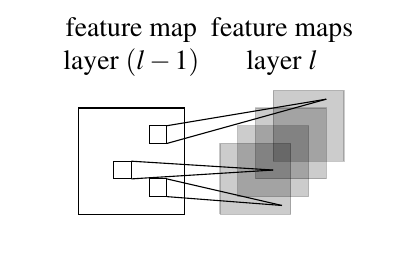
\begin{tikzpicture}[scale=0.45]
		    \node at (1.5,4.75){\begin{tabular}{c}feature map\\layer $(l - 1)$\end{tabular}};
	
		    \draw (0,0) -- (3,0) -- (3,3) -- (0,3) -- (0,0);
		
		    \draw (2,2) -- (2.5,2) -- (2.5,2.5) -- (2,2.5) -- (2,2);
		    \draw (2,0.5) -- (2.5,0.5) -- (2.5,1) -- (2,1) -- (2,0.5);
		    \draw (1,1) -- (1.5,1) -- (1.5,1.5) -- (1,1.5) -- (1,1);
		
		    \draw (2.5,2) -- (7,3.25);
		    \draw (2.5,2.5) -- (7,3.25);

		    \draw (2.5,1) -- (5.75,0.25);
		    \draw (2.5,0.5) -- (5.75,0.25);
		
		    \draw (1.5,1.5) -- (5.5,1.25);
		    \draw (1.5,1) -- (5.5,1.25);
		
		    \node at (5.75,4.75){\begin{tabular}{c}feature maps\\layer $l$\end{tabular}};
		
		    \draw[fill=black,opacity=0.2,draw=black] (5.5,1.5) -- (7.5,1.5) -- (7.5,3.5) -- (5.5,3.5) -- (5.5,1.5);
		    \draw[fill=black,opacity=0.2,draw=black] (5,1) -- (7,1) -- (7,3) -- (5,3) -- (5,1);
		    \draw[fill=black,opacity=0.2,draw=black] (4.5,0.5) -- (6.5,0.5) -- (6.5,2.5) -- (4.5,2.5) -- (4.5,0.5);
		    \draw[fill=black,opacity=0.2,draw=black] (4,0) -- (6,0) -- (6,2) -- (4,2) -- (4,0);
	    \end{tikzpicture}
	}
	\subfigure[\label{subfig:local-contrast-layer}]{
	    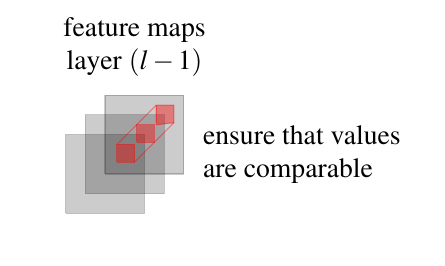
\begin{tikzpicture}[scale=0.5]
	        \node at (1.75,4.25){\begin{tabular}{c}feature maps\\layer $(l - 1)$\end{tabular}};
	        
			\draw[fill=black,opacity=0.2,draw=black] (1,1) -- (3,1) -- (3,3) -- (1,3) -- (1,1);
			\draw[fill=black,opacity=0.2,draw=black] (0.5,0.5) -- (2.5,0.5) -- (2.5,2.5) -- (0.5,2.5) -- (0.5,0.5);
			\draw[fill=black,opacity=0.2,draw=black] (0,0) -- (2,0) -- (2,2) -- (0,2) -- (0,0);
			
			\draw[opacity=0.4,draw=red,fill=red] (2.3,2.25) -- (2.75,2.3) -- (2.75,2.75) -- (2.3,2.75) -- (2.3,2.3);
			\draw[opacity=0.4,draw=red,fill=red] (1.8,1.8) -- (2.25,1.8) -- (2.25,2.25) -- (1.8,2.25) -- (1.8,1.8);
			\draw[opacity=0.4,draw=red,fill=red] (1.3,1.3) -- (1.75,1.3) -- (1.75,1.75) -- (1.3,1.75) -- (1.3,1.3);
			\draw[opacity=0.4,draw=red](1.3,1.75) --  (1.8,2.25);
			\draw[opacity=0.4,draw=red](1.75,1.3) -- (2.25,1.8);
			\draw[opacity=0.4,draw=red](2.25,1.8) -- (2.75,2.3);
			\draw[opacity=0.4,draw=red](1.8,2.25) -- (2.3,2.75);
			
			\node at (6,1.5){\begin{tabular}{l}ensure that values\\are comparable\end{tabular}};
		\end{tikzpicture}
	}
	\subfigure[\label{subfig:pooling-layer}]{
	    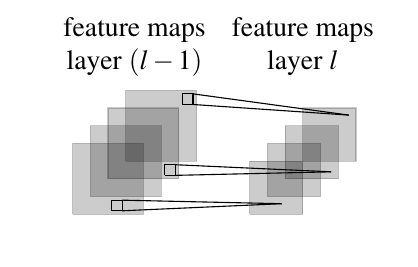
\begin{tikzpicture}[scale=0.45]
		    \node at (1.75,4.75){\begin{tabular}{c}feature maps\\layer $(l-1)$\end{tabular}};
		
		    \draw[fill=black,opacity=0.2,draw=black] (1.5,1.5) -- (3.5,1.5) -- (3.5,3.5) -- (1.5,3.5) -- (1.5,1.5);
		    \draw[fill=black,opacity=0.2,draw=black] (1,1) -- (3,1) -- (3,3) -- (1,3) -- (1,1);
		    \draw[fill=black,opacity=0.2,draw=black] (0.5,0.5) -- (2.5,0.5) -- (2.5,2.5) -- (0.5,2.5) -- (0.5,0.5);
		    \draw[fill=black,opacity=0.2,draw=black] (0,0) -- (2,0) -- (2,2) -- (0,2) -- (0,0);
		
		    \draw (3.1,3.1) -- (3.4,3.1) -- (3.4,3.4) -- (3.1,3.4) -- (3.1,3.1);
		    \draw (2.6,1.1) -- (2.9,1.1) -- (2.9,1.4) -- (2.6,1.4) -- (2.6,1.1);
		    \draw (1.1,0.1) -- (1.4,0.1) -- (1.4,0.4) -- (1.1,0.4) -- (1.1,0.1);
		
		    \draw (3.4,3.4) -- (7.8,2.8);
		    \draw (3.4,3.1) -- (7.8,2.8);
		
		    \draw (2.9,1.4) -- (7.3,1.2);
		    \draw (2.9,1.1) -- (7.3,1.2);
		
		    \draw (1.4,0.4) -- (5.9,0.3);
		    \draw (1.4,0.1) -- (5.9,0.3);
		
		    \node at (6.5,4.75){\begin{tabular}{c}feature maps\\layer $l$\end{tabular}};
		
		    \draw[fill=black,opacity=0.2,draw=black] (6.5,1.5) -- (8,1.5) -- (8,3) -- (6.5,3) -- (6.5,1.5);
		    \draw[fill=black,opacity=0.2,draw=black] (6,1) -- (7.5,1) -- (7.5,2.5) -- (6,2.5) -- (6,1);
		    \draw[fill=black,opacity=0.2,draw=black] (5.5,0.5) -- (7,0.5) -- (7,2) -- (5.5,2) -- (5.5,0.5);
		    \draw[fill=black,opacity=0.2,draw=black] (5,0) -- (6.5,0) -- (6.5,1.5) -- (5,1.5) -- (5,0);
	    \end{tikzpicture}
	}
	\caption{Illustration of a \ref{subfig:convolutional-layer} convolutional layer; \ref{subfig:local-contrast-layer} local contrast normalization layer; and \ref{subfig:pooling-layer} pooling layer.}
	\label{fig:convolutional-layer}
\end{figure}

\subsubsection{Pooling Layer}
\label{subsubsec:pooling-layer}

While LeCun \etal \cite{LeCunBoserDenkerhendersonHowardHubbardJackel:1989} use subsampling within convolutional layers (that is, the convolution in Equation \eqref{eq:convolutional-layer} is not applied on every entry of the input feature maps), recent architectures prefer to use separate pooling layers to reduce the size of the feature maps and introduce invariance to noise and distortions. Similar to the aggregation step of local descriptors used by Ge \etal \cite{GeKeSun:2013}, max pooling or average pooling are common:
\vspace{-6px}
\begin{description}
	\item[Average pooling] computes the average value within (non-overlapping) windows; while
	\vspace{-14px}
	\item[Max pooling] computes the maximum value within (non-overlapping) windows.
\end{description}
\vspace{-6px}
Pooling has been found to improve convergence and reduce overfitting \cite{KrizhevskySutskeverHinton:2012}. Note that pooling can also be used with overlapping filters, see \cite{KrizhevskySutskeverHinton:2012}.

\subsubsection{Fully-Connected Layer}
\label{subsubsec:fully-connected}

If layer $l$ is a fully connected layer and layer $(l - 1)$ one of the above layers, the input feature maps $Y_i^{(l-1)}$ are interpreted as $m_2^{(l-1)} \cdot m_3^{(l-1)}$-dimensional vectors and layer $l$ computes:
\begin{align}
    y_i^{(l)} = f\left(z_i^{(l)}\right) = f\left(\sum_{j = 1}^{m_1^{(l-1)}} \sum_{r = 1}^{m_2^{(l-1)}} \sum_{s = 1}^{m_3^{(l-1)}} w_{i,j,r,s}^{(l)} \left(Y_j^{(l-1)}\right)_{r,s}\right),\quad \forall 1 \leq i \leq m^{(l)}\label{eq:fully-connected}.
\end{align}
Note that, in contrast to convolutional layers, this layer already includes non-linearities. In the case that layer $(l-1)$ is a fully connected layer, Equation \eqref{eq:fully-connected} can be applied analogously to Equation \eqref{eq:neural-network}.
%\begin{align}
%    y_i^{(l)} = f\left( \sum_{j = 1}^{m^{(l-1)}} w^{(l)}_{i,j} y_j^{(l - 1)} + w^{(l)}_{i,0}\right),\quad 1 \leq i \leq m_1^{(l)}\label{eq:fully-connected-simple}.
%\end{align}
In convolutional neural networks, both layer $(L - 1)$ and layer $L$ are usually fully connected layers and layer $L$ uses the softmax activation function and is used for classification.

\subsection{Architectures}
\label{subsec:architectures}

Most architectures used in practice can be described using the layer types discussed above (for example \cite{LeCunBoserDenkerhendersonHowardHubbardJackel:1989,JarrettKavukcuogluRanzatoLeCun:2009}). For example, the architecture introduced by Krizhevsky \etal can be described as follows. Five convolutional layers with rectified linear unit non-linearity layers are followed by three fully connected layers
\footnote{
    The exact architecture can also be seen when consulting the reference model shipped with Caffe \cite{JiaShelhamerDonahueKarayevLongGirshickGuadarramaDarrell:2014}, see Section \ref{sec:implementations}. Note that Caffe requires some extra layer types for training as well as pre-processing and includes dropout regularization, discussed in Section \ref{subsubsec:regularization}, as additional layer type.
}.
Local contrast normalizaton layers are used after the first and second non-linearity layers (corresponding to the first and second convolutional layers). Overlapping max pooling layers are used after the first and second contrast normalization layer as well as after the fifth non-linearity layer. Although not formalized in Section \ref{subsubsec:convolutional-layer}, the convolutional layers are not necessarily fully connected to the previous layers, that is the sum in Equation \eqref{eq:convolutional-layer} does not run over all input feature maps. This is due to computational reasons, see \cite{KrizhevskySutskeverHinton:2012}. The last layer uses softmax activation functions. Figure \ref{fig:architecture} shows the overall architecture including the specific fiilter and feature map sizes.
% Overall, these are $18$ layers with $y^{(18)}$ being the posterior probabilities and $y^{(17)}$, $y^{(16)}$ the previous fully connected layers.
\begin{figure}
	\centering
	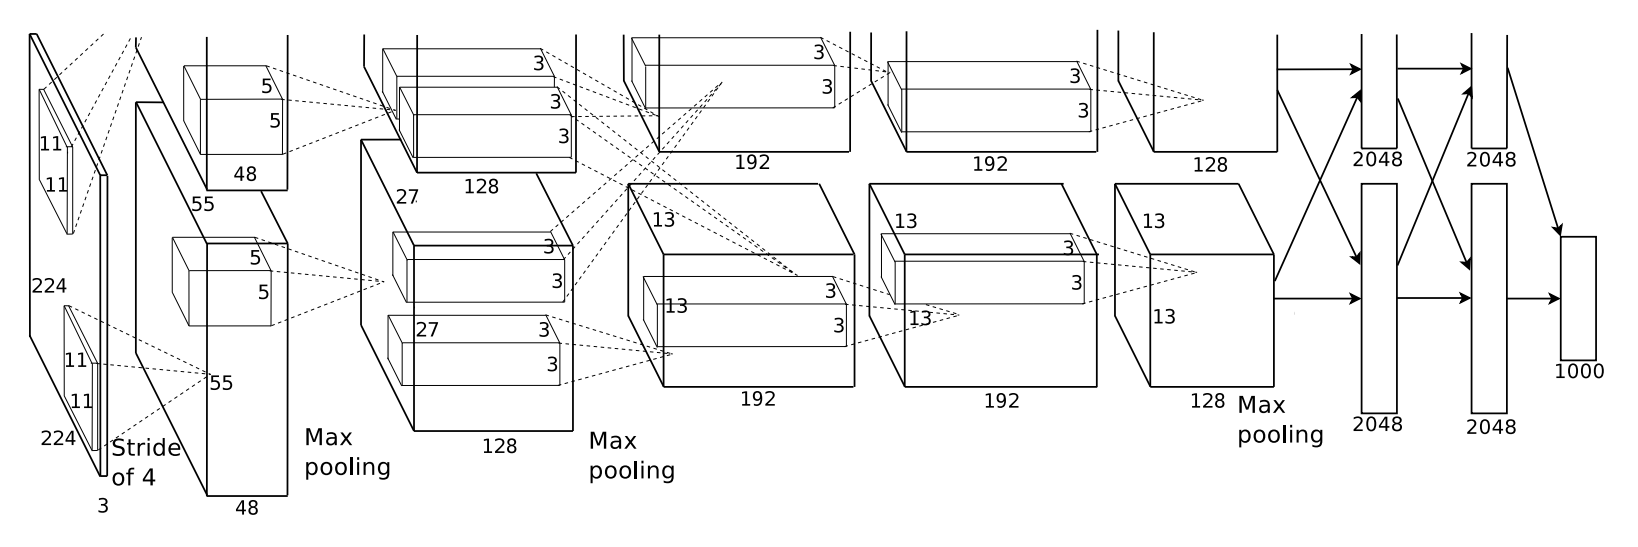
\includegraphics[scale=0.4]{pictures/architecture}
	\caption{The architecture used by Krizhevsky \etal \cite{KrizhevskySutskeverHinton:2012}. The number $m_1^{(l)}$ of computed feature maps in layer $l$ is indicated by the width of the corresponding cuboid, while the size $m_2^{(l)} \times m_3^{(l)}$ of the feature maps is indicated by the height and depth, respectively. In addition, the size of the filters $W_{i,j}^{(l)}$ is shown. For example, the input is given by a single gray-scale image of size $244 \times 244$. Using filters of size $11 \times 11$, the first convolutional layer computes $96 = 48 + 48$ feature maps of size $55 \times 55$. Furthermore, the filters in the first convolutional layer are applied in strides of $4$ pixels. We note that the architecture has been parallelized and refer to \cite{KrizhevskySutskeverHinton:2012} for details.}
	\label{fig:architecture}
\end{figure}

\subsection{Available Implementations}
\label{sec:implementations}

The main problem of implementing and training deep convolutional neural networks is computational efficiency. Therefore, most implementations use one or more GPUs. For example, the original implementation by Krizhevsky \etal uses two Nvidida GTX 580
\footnote{
    The implementation is available at \url{http://www.cs.toronto.edu/~kriz/}.
} -- still, training on the ImageNet dataset \cite{DengDongSocherLiLiLi:2009} took several days. As a result, pre-trained models have become quite popular (that is, the weights of a trained network together with a specification of the network architecture are shared with the community).
This is simplified by publicly available frameworks as for example Caffe \cite{JiaShelhamerDonahueKarayevLongGirshickGuadarramaDarrell:2014}, which comes with several pre-trained models using different architectures.
Another popular convolutional neural network library is OverFeat
\footnote{
    Available at \url{http://cilvr.nyu.edu/doku.php?id=code:start}.
}.
% Further, since the success by Krizhevsky \etal \cite{KrizhevskySutskeverHinton:2012}, frameworks for deep learning on various platforms and using different programming languages (for example Mocha, written in Julia
% \footnote{
    % Mocha is a deep learning framework for Julia, a young (2012) programming language designed for scientific computing. See \url{https://github.com/pluskid/Mocha.jl}.
% }) have been created and are gaining popularity across the borders of computer vision
% \footnote{
    % We refer to \url{http://deeplearning.net/software_links/} for a complete list of available implementations.
% }.

\subsection{Training}
\label{subsec:training}

Training convolutional neural networks means to adjust the weights $\mathbf{W} = \{w_{i,j,r,s}^{(l)}\}$ according to a loss applied on layer $L$. Given a training set $\{(x_1,t_1),\ldots,(x_N,t_N)\}$ with $t_n \in \{1,\ldots,m^{(L)}\}$ being class labels, common loss functions for classification include the sum-of-squared error and the cross-entropy error.
Instead, Krizhevsky \etal minimize the multinomial logistic loss:
\begin{align}
    E(\mathbf{W}) = - \frac{1}{m^{(L)}} \sum_{n = 1}^{N} log\left(y_{t_n}^{(L)}\right)\label{eq:multinomial-loss}
\end{align}
where $y_{t_n}^{(L)}$ is expected to model the posterior probability $p(t_n | x_n)$ of sample $x_n$ belonging to class $t_n$. These loss functions can be defined on the whole training set, as in Equation \eqref{eq:multinomial-loss}, on so-called mini-batches, that is on small subsets of the training set, or on individual training examples. Therefore, convolutional neural networks can also be trained online.

A common algorithm used for minimization is gradient descent, an iterative technique which, starting with an initial guess $\mathbf{W}[0]$, iteratively takes steps in the direction of the negative gradient (that is, the direction of the steepest descent in $L_2$ norm). Following \cite{Bottou:2012}, and given a learning rate $\gamma$, gradient descent is implemented using the update step
\begin{align}
    \mathbf{W}[\tau + 1] = \mathbf{W}[\tau] - \gamma \nabla E\left(\mathbf{W}[\tau]\right)\label{eq:gradient-descent}.
\end{align}
The chosen learning rate $\gamma$ is crucial and usually has strong influence on the found minima. A widely used extension is gradient descent with momentum term which aims to avoid oscillation while using a high learning rate for fast training. The update step changes to:
\begin{align}
    \mathbf{W}[\tau + 1] = \mathbf{W}[\tau] - \gamma \nabla E\left(\mathbf{W}[\tau]\right) + \nu(\mathbf{W}[\tau] - \mathbf{W}[\tau - 1])
\end{align}
where $\nu$ is the momentum parameter.
% In practice, the learning rate may be depending on the iteration (that is, manually or automatically adapted during the training process).

Stochastic gradient descent applies the update of Equation \eqref{eq:gradient-descent} on a subset of randomly selected samples. It can be shown that stochastic gradient descent converges under relatively loose conditions \cite{Bottou:2012}. In addition, stochastic gradient descent may be beneficial for large-scale learning \cite{Bottou:2012} and improve the generalization performance of the learned model \cite{BottouBousquet:2007}. 
% Krizhevsky \etal \cite{KrizhevskySutskeverHinton:2012} additionally use weight decay, see Section \ref{subsubsec:regularization}.

For applying stochastic gradient descent, the gradient $\nabla E(\mathbf{W}[\tau])$ needs to be computed in each iteration. Therefore, Error Backpropagation has been proposed and allows to compute the gradient $\nabla E(\mathbf{W}[\tau])$ in~$\mathcal{O}\left(|\mathbf{W}|\right)$ \cite{Bishop:1995}.

%\subsubsection{Deep Training}
%\label{subsubsec:deep-training}

\subsubsection{Regularization}
\label{subsubsec:regularization}

Regularization is used to control the complexity of the model during training to prevent overfitting. For example, Krizhevsky \etal use weight decay and dropout as regularization during training. Weight decay is simple $L_2$-normalization of the weights and used because large weights result in poor generalization~\cite{Bishop:1995}. The updated loss function can be written as:
\begin{align}
    \hat{E}(\mathbf{W}) = E(\mathbf{W}) + \lambda \|\mathbf{W}\|_2.
\end{align}
In contrast, dropout \cite{KrizhevskySutskeverHinton:2012} tries to decouple pairs of computation units (that is individual elements within the feature maps $Y_i^{(l)}$ or the computed vectors $y^{(l)}$). Each such unit is deactivated (that is, set to zero) with probability one half. The intention is to avoid subsequent layers or neighboring units being dependent on specific units.

	\section{Neural Codes for Image Retrieval}
\label{sec:neural-codes-image-retrieval}

As discussed in \cite{Bengio:2009}, convolutional neural networks tend to learn useful high- and mid-level filters and the generated activations are rich representations of image content. Therefore, convolutional neural networks have been applied to many different tasks. Babenko \etal \cite{BabenkoSlesarevChigorinLempitsky:2014} use the generated feature activations as image representation for image retrieval. The resulting image representations are also termed neural codes.

\subsection{Architecture, Training and Implementation}

According to Babenko \etal, the same architecture as presented in Section \ref{subsec:architectures} was used together with an adapted version of the original implementation by Krizhevsky \cite{KrizhevskySutskeverHinton:2012} \etal.
Experiments were conducted using a model pre-trained on the ImageNet dataset \cite{DengDongSocherLiLiLi:2009} and a model re-trained on a custom dataset consisting of popular landmarks (referred to as the Landmark dataset).
The dataset comprises $213,678$ images with $672$ classes (corresponding to the different landmarks) and was collected using the Yandex search engine
\footnote{
    See \url{https://www.yandex.com/}.
}.
Although, the search queries have been published
\footnote{
    Available at \url{http://sites.skoltech.ru/compvision/projects/neuralcodes} (in Russian).
}, the dataset is not directly reproducible. Furthermore, the implementation has not been made publicly available.

Training is done according to \cite{KrizhevskySutskeverHinton:2012}, see Section \ref{subsec:training}, using stochastic gradient descent with a momentum parameter $\nu = 0.9$ and weight decay with $\lambda = 0.0005$. The learning rate is initialized with $\gamma = 0.01$ and manually divided by $10$ whenever the error on a validation set stops decreasing. As Babenko \etal do not mention deviations from this procedure, we assume that the same approach was used for the re-trained model.

\subsection{Compression}
\label{subsec:compression}

The feature activations in intermediate layers may be quite high-dimensional. Thus, Babenko \etal \cite{BabenkoSlesarevChigorinLempitsky:2014} experiment with two different approaches for dimensionality reduction: \textbf{PCA} and metric learning following the idea of \cite{SimonyanParkhiVedaldiZisserman:2013}.

\vskip 6px
\textbf{Large-Margin Dimensionality Reduction} \cite{SimonyanParkhiVedaldiZisserman:2013}. Babenko \etal collect a dataset of $100k$ image pairs from the Landmark dataset using a simple image matching system (\textbf{SIFT} matching with Lowe's ratio test \cite{Lowe:2004} and \textbf{RANSAC} validation). The goal is to learn a linear dimensionality reduction $P \in \mathbb{R}^{C' \times C}$ such that the distance of matching image pairs is below a learned threshold $b$ while the distance of non-matching pairs is above this threshold. This can be formalized by the constraint
\begin{align}
    t_{n,n'} \left(b - d(P x_n, P x_{n'})^2\right) > 1
\end{align}
where $t_{n,n'} = 1$ if and only if the image pair $(x_n, x_{n'})$ is a matching pair. This can be accomplished by minimizing 
\begin{align}
    E(P) = \sum_{n,n'}^N \max\{0, 1 - t_{n,n'}\left(b - (x_n - x_{n'})^T P^T P (x_n - x_{n'})\right)\}
\end{align}
using stochastic gradient descent. In particular, given a sampled pair of image representations $(x_n, x_{n'})$ the dimensionality reduction $P[\tau]$ in iteration $\tau$ is updated only if
\begin{align}
    t_{n,n'} \left(b - (x_n - x_{n'})^T P[\tau]^T P[\tau] (x_n - x_{n'})\right) > 1
\end{align}
and according to
\begin{align}
	P[\tau + 1] = P[\tau] - \gamma  t_{n,n'} P[\tau] (x_n - x_{n'})(x_n - x_{n'})^T
\end{align}
where $\gamma$ is the learning rate. Instead of an additional regularization term, Simonyan \etal use early stopping, that is minimization is stopped after a pre-defined number of iterations. Positive and negative pairs are sampled with equal probability.

	\section{Experiments}
\label{sec:experiments}

In this section, we discuss several experiments presented by Babenko \etal \cite{BabenkoSlesarevChigorinLempitsky:2014}. However, first we introduce popular datasets and the general evaluation methodology employed in the image retrieval community.

\subsection{Datasets}

There are several commonly used datasets available within the image retrieval community.
% Note that the evaluation methodology may differ between datasets.
We briefly discuss two datasets used for evaluation of many approaches discussed in Section \ref{subsubsubsec:local-descriptors}.
% TODO: links to datasets.
\vskip 6px
\textbf{Oxford 5k (+100k, +1M)} \cite{PhilbinChumIsardSivicZisserman:2007}. The Oxford dataset consists of $5,062$ images showing eleven different Oxford landmarks. The images were retrieved from Flickr
\footnote{
    See \url{https://www.flickr.com/}.
} by querying directly for these landmarks and adding several distractor images using the query ``Oxford'' alone. For each landmark five queries are provided and for each query, four different lists are available: ``Good'', that is the queried object is visible in the image; ``Ok'', that is most of the object (more than $25\%$) is visible; ``Junk'', that is the object is heavily occluded (less than $25\%$ visible); and ``Absent'', that is the object is not shown in the image. Furthermore, two set of distractor images are provided: $99,782$ images from the $145$ most popular tags on Flickr (+100k); and  $1,040,801$ images from the $450$ most popular tags on Flickr (+1M). Duplicates with the original 5k datasets have been removed.

\vskip 6px
\textbf{INRIA Holidays} \cite{JegouDouzeSchmid:2008}. The dataset comprises $1,491$ personal holiday images and comes with $500$ distinct queries including ground truth results. Some of the images were taken explicitly to test the system against illumination changes and viewpoint changes. However, Babenko \etal manually bring all images in the correct orientation.

%\vskip 6px
%\textbf{University of Kentucky Dataset} \cite{NisterStewenius:2006}. The dataset contains $2,550$ objects with $4$ images per object. Each image can be used as query and performance is measures as fraction of correct retrieval results in the top-4 images.

\subsection{Mean Average Precision}

Performance evaluation is usually based on a fixed number $K$ of retrieved images per query. Given a query $z_0$ and retrieved images $Z = (z_1,\ldots,z_K)$, we define:

\vskip 6px
\textbf{True Positives} $TP$: the number of images retrieved that are relevant to the query (that is, show the same object or scene);\\
\textbf{False Positives} $FP$: the number of images retrieved that are not relevant to the query;\\
\textbf{False Negatives} $TN$: the number of images which are relevant to the query but not retrieved.
\vskip 6px

Then, Precision and Recall are given as
\begin{align}
    \text{Pre}(Z) = \frac{TP}{TP + FP}\quad\text{ and }\quad \text{Rec}(Z) = \frac{TP}{TP + FN}.
\end{align}
The Precision-Recall curve is a common instrument to visualize and understand the performance of a retrieval systems. Furthermore, this curve can be summarized in a single value: Average Precision which can be interpreted as the area under the curve. Let $\text{Pre}_k(Z)$ and $\text{Rec}_k(Z)$ be Precision and Recall up to the $k$-th retrieved image, respectively. Then, Average Precision is computed as
\footnote{
    See the provided source code at \url{http://www.robots.ox.ac.uk/~vgg/data/oxbuildings/}.
}
\begin{align}
    \text{AP}(Z) = \sum_{k = 1}^K (\text{Rec}_k(Z) - \text{Rec}_{k-1}(Z))\frac{(\text{Pre}_{k-1}(Z) + \text{Pre}_k(Z))}{2}
\end{align}
with $\text{Rec}_0(Z) = 0$ and $\text{Pre}_0(Z) = 1$. The Mean Average Precision is calculated to report the performance over a set of queries.

\subsection{Results}

As Babenko \etal do not provide the used implementation or the Landmark dataset, we were not able to reproduce their experimental results. Therefore, Table \ref{table:pre-re-trained} summarizes results reported in \cite{BabenkoSlesarevChigorinLempitsky:2014}. In particular, they experiment with three distinct layers for image representation: $y^{(15)}$ corresponds to the last convolutional layer including the subsequent non-linearity layer and max pooling layer; $y^{(16)}$ and $y^{(17)}$ correspond to the first and second fully connected layer. On the Oxford 5k dataset, the pre-trained model shows poor performance and the re-trained model is not able to cope with the approach by J{\'e}gou and Zisserman \cite{JegouZisserman:2014}. In contrast, both the pre-trained model and the re-trained model demonstrate state-of-the-art performance on the Holidays dataset. Further, we see that layer $16$ performs best.
% Babenko \etal argue that this might be due to the fact that the last layers are increasingly tuned towards the classification task.

As discussed in Section \ref{subsec:compression}, Babenko \etal experiment with \textbf{PCA} and Large-Margin Dimensionality Reduction and Table \ref{table:compression} shows the corresponding results. On both the Oxford 5k dataset and the Holidays dataset, the feature activations seem to be more robust to dimensionality reduction. Compared to the other approaches, also using \textbf{PCA} for dimensionality reduction, the compressed re-trained feature activations show significantly better performance. However, we also note that Large-Margin Dimensionality Reduction does not show a significant advantage over \textbf{PCA}. Lastly, figure \ref{fig:qualitative} shows two retrieval examples.

\begin{SCtable}[2][t]
    \centering
    {
    \footnotesize
    \def\arraystretch{1.1}
    \begin{tabular}{| l | r | r |}
        \hline
        & Oxford 5k & Holidays\\\hline
        \cite{GordoSerranoPerronninValveny:2012} & -- & 0.774\\
        \cite{ArandjelovicZisserman:2013} & 0.555 & 0.646\\
        \cite{GeKeSun:2013} & -- & 0.767\\
        \cite{JegouZisserman:2014} & 0.676 & 0.771\\\hline
        \multicolumn{3}{| c |}{\textbf{Pre-Trained on ImageNet \cite{DengDongSocherLiLiLi:2009}}}\\\hline
        $y^{(15)}$ & 0.389 & 0.69\\
        $y^{(16)}$ & 0.435 & 0.749\\
        $y^{(17)}$ & 0.430 & 0.736\\\hline
        \multicolumn{3}{| c |}{\textbf{Re-Trained}}\\\hline
        $y^{(15)}$ & 0.387 & 0.674\\
        $y^{(16)}$ & 0.545 & 0.793\\
        $y^{(17)}$ & 0.538 & 0.764\\\hline
    \end{tabular}
    }
    \caption{Mean average precision for the Oxford 5k dataset and the Holidays dataset. Using the notation from Section \ref{sec:convolutional-neural-networks}, Babenko \etal use $y^{(17)}$, $y^{(16)}$ and $y^{(15)}$ as image representations. These layer correspond to the second and first fully connected layers, each with dimension $C = 4096$, and the last convolutional layer including non-linearity layer and max pooling layer, resulting in $C = 9216$. The results are compared to the following approaches: Gordo \etal \cite{GordoSerranoPerronninValveny:2012} use Fisher Vectors on densily extracted \textbf{SIFT} descriptors; Arandjelovi{\'c} and Zisserman \cite{ArandjelovicZisserman:2013} use \textbf{VLAD} with intra-normalization; Ge \etal \cite{GeKeSun:2013} use sparse-coding to combine \textbf{SIFT}, \textbf{DAISY} \cite{TolaLepetitFua:2008} and Sparse-Coded Micro Features; and J{\'e}gou and Zisserman \cite{JegouZisserman:2014} use Triangulation Embedding and Democratic Aggregation.}
    \label{table:pre-re-trained}
\end{SCtable}

\begin{SCtable}[2][b]
    \centering
    {
    \footnotesize
    \def\arraystretch{1.1}
    \begin{tabular}{| l | r | r |}
        \hline
        & Oxford 5k & Holidays\\\hline
        \cite{GordoSerranoPerronninValveny:2012} & -- & 0.723\\
        \cite{GordoSerranoPerronninValveny:2012}* & -- & 0.764\\
        \cite{ArandjelovicZisserman:2013} & 0.448 & 0.625\\
        \cite{GeKeSun:2013} & -- & 0.727\\
        \cite{JegouZisserman:2014} & 0.433 & 0.617\\\hline
        \multicolumn{3}{| c |}{\textbf{Pre-Trained on ImageNet \cite{DengDongSocherLiLiLi:2009}}}\\\hline
        $y^{(16)}$ (\textbf{PCA}) & 0.433 & 0.747\\
        $y^{(16)}$ (Large-Margin) & 0.439 & --\\\hline
        \multicolumn{3}{| c |}{\textbf{Re-Trained}}\\\hline
        $y^{(16)}$ (\textbf{PCA})& 0.557 & 0.789\\
        \hline
    \end{tabular}
    }
    \caption{Mean average precision for the Oxford 5k dataset and the Holidays dataset using $128$ dimensional image representations. Babenko \etal use layer $y^{(16)}$ (as it experimentally yields the best results) compressed to $128$ dimensions using \textbf{PCA} and Large-Margin Dimensionality Reduction. The other approaches have been compressed as discussed in the corresponding publications: Gordo \etal \cite{GordoSerranoPerronninValveny:2012} use \textbf{PCA} and Joint Subspace and Classifier Learning (marked with *); Arandjelovi{\'c} and Zisserman \cite{ArandjelovicZisserman:2013} use \textbf{PCA}; Ge \etal \cite{GeKeSun:2013} use \textbf{PCA}; and J{\'e}gou and Zisserman \cite{JegouZisserman:2014} use power-law normalization after \textbf{PCA} rotation and subsequently keep the first $128$ dimensions (see \cite{JegouZisserman:2014} for details).}
    \label{table:compression}
\end{SCtable}

\subsection{Discussion}

The experiments by Babenko \etal raise several questions. First of all, the choice of layer is only justified experimentally and the re-trained convolutional neural network has been trained towards the classification task, as well. Only in the conclusion, Babenko \etal consider training the network directly on image pairs. Second, Large-Margin Dimensionality Reduction has not been demonstrated on the re-trained neural network. As the approach does not demonstrate any significant increase in performance over \textbf{PCA} on the pre-trained model, this may imply that discriminative dimensionality reduction does not work well for convolutional neural networks. However, we note that Gordo \etal are able to significantly increase performance using Joint Subspace and Classifier Learning -- a comparison not available in \cite{BabenkoSlesarevChigorinLempitsky:2014}. Finally, results for the compared approaches shown in Tables \ref{table:pre-re-trained} and \ref{table:compression} are taken from the corresponding publications and Babenko \etal do not discuss the used evaluation pipeline in detail such that the reported results may not be comparable.
% The experiments by Babenko \etal \cite{BabenkoSlesarevChigorinLempitsky:2014} show mixed results. While the re-trained convolutional neural network demonstrates excellent performance on the Holidays dataset, results on the Oxford 5k dataset are not able to cope with the state-of-the-art (that is \cite{JegouZisserman:2014}). In contrast, feature activations from convolutional neural networks seem to be more robust to \textbf{PCA} compression (at least compared to \cite{GordoSerranoPerronninValveny:2012,ArandjelovicZisserman:2013,GeKeSun:2013} also using \textbf{PCA}). Furthermore, Babenko \etal argue that the last layers of a convolutional neural network are tuned towards the classification task justifying the use of intermediate layers for image representation. However, this has only been shown experimentally and the compression of additional intermediate layers has not been considered. In addition, the re-trained convolutional neural network has specificly been trained on a classification task, as well. Only in their conclusion, Babenko \etal consider training the convolutional neural network directly on image pairs \cite{BabenkoSlesarevChigorinLempitsky:2014}.

	\begin{figure}
    \centering
    % 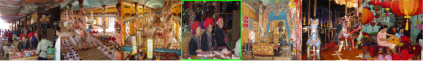
\includegraphics[scale=0.6]{pictures/qualitative-row-1}
    % 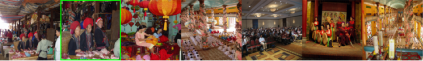
\includegraphics[scale=0.6]{pictures/qualitative-row-2}
    % 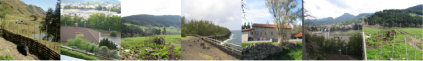
\includegraphics[scale=0.6]{pictures/qualitative-row-5}
    % 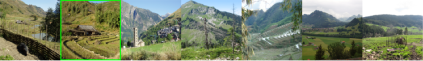
\includegraphics[scale=0.6]{pictures/qualitative-row-6}
    % 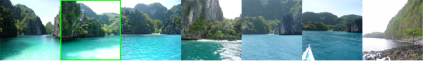
\includegraphics[scale=0.6]{pictures/qualitative-row-7}
    % 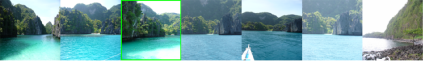
\includegraphics[scale=0.6]{pictures/qualitative-row-8}
    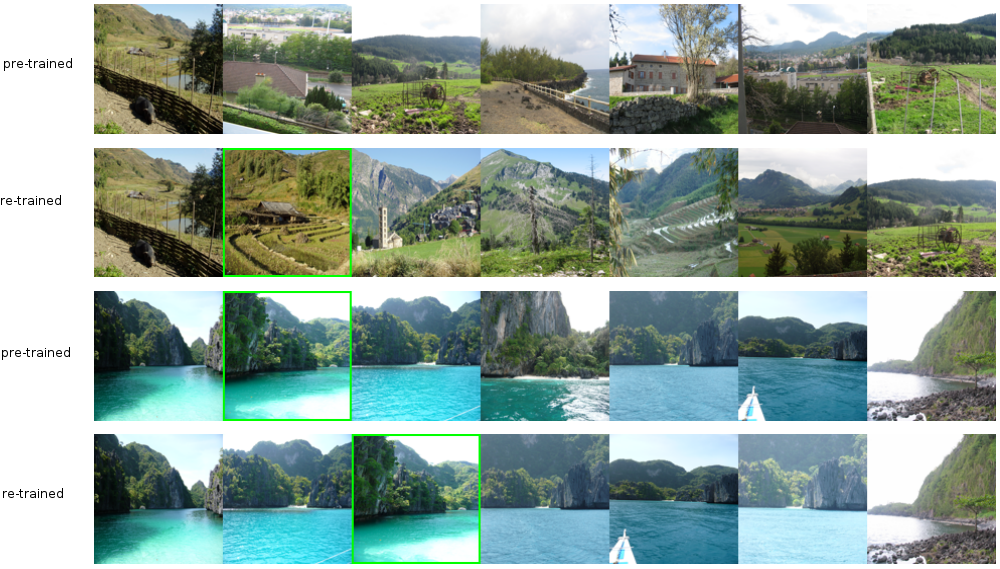
\includegraphics[scale=0.4]{pictures/qualitative-annotated}
    \caption{Two retrieval examples (taken from \cite{BabenkoSlesarevChigorinLempitsky:2014}) on the Holidays dataset using the pre-trained model (on the top, respectively) and the re-trained model (on the bottom, respectively). In each row, the left-most image is the query image and correctly retrieved images are outlined in green. Babenko \etal point out that the lower example is a ``rare exception'' \cite[p. 10]{BabenkoSlesarevChigorinLempitsky:2014} where the pre-trained model outperforms the re-trained model.}
    \label{fig:qualitative}
\end{figure}

\section{Conclusion}
\label{sec:conclusion}

In the course of this report we presented current techniques in content-based image retrieval. In particular, we discussed local descriptors and their aggregation techniques in Section \ref{subsubsec:local-descriptors}, as well as global descriptors in Section \ref{subsubsec:global-descriptors}. Furthermore, after discussing convolutional neural networks in Section \ref{sec:convolutional-neural-networks}, we discussed the use of convolutional neural networks in image retrieval in Section \ref{sec:neural-codes-image-retrieval}. Finally, we presented experimental results following Babenko \etal \cite{BabenkoSlesarevChigorinLempitsky:2014} in Section \ref{sec:experiments}.

Overall, we discussed many approaches related to the Bag of Visual Words model \cite{SivicZisserman:2003} relying mostly on hand-crafted descriptors. Although some techniques make use of metric learning or similar (supervised or unsupervised) learning techniques, the embedding step and/or the aggregation step are heavily guided by manual processes, that is the whole retrieval system is explicitly engineered by hand.
% This includes all subproblems discussed in Section \ref{sec:image-retrieval}: local descriptors, normalization, embedding and aggregation.
In strong contrast, Babenko \etal use convolutional neural networks to automatically learn most of these tasks. Although, the presented results are not fully convincing, especially on the Oxford 5k dataset \cite{PhilbinChumIsardSivicZisserman:2007}, this approach opens a new direction of research where several subproblems are solved fully by learning algorithms. Still, the image retrieval community will try to improve these results by adapting pre- or post-processing as well as network architecture.

\subsection{Research Questions}

We conclude that combining hand-crafted approaches with convolutional neural networks may be a promising future research direction. For example, different normalization techniques (for example \cite{ArandjelovicZisserman:2013}) may improve performance. Furthermore, layer selection has only be done experimentally based on the mean average precision. In contrast, visualizing the energy of the image representations as done in \cite{ArandjelovicZisserman:2013} may help to select suitable layers. In addition, the convolutional neural network was explicitly trained in a classification framework. Other architectures, as for example a Siamese architecture (see \cite{BabenkoSlesarevChigorinLempitsky:2014} for references), may be tailored directly towards the image retrieval task. Finally, techniques allowing to combine the information of multiple layers similar to \cite{GeKeSun:2013} may be interesting.


	\bibliographystyle{alpha}
	\bibliography{seminar}
\end{document}
